\documentclass[12pt]{article}
\usepackage{amsmath,amssymb,amsfonts,amsthm}
\usepackage{graphicx}
\usepackage{hyperref}
\usepackage{geometry}
\usepackage{authblk}
\usepackage{cite}
\usepackage{enumitem}
\usepackage{mathrsfs}

\geometry{margin=1in}

\newtheorem{theorem}{Theorem}
\newtheorem{lemma}{Lemma}
\newtheorem{proposition}{Proposition}
\newtheorem{corollary}{Corollary}
\theoremstyle{definition}
\newtheorem{definition}{Definition}
\newtheorem{assumption}{Assumption}
\newtheorem{remark}{Remark}

\title{Observer-Interface Emergence of Formal Systems and Scale-Relative Informational Persistence}
\author{Christopher Ezernack}
\date{}

\begin{document}

\maketitle

\begin{abstract}
This paper introduces a formal framework in which mathematical and informational structures are not treated as intrinsic properties of an absolute reality, but as emergent properties of an observer interface interaction. We define coherence, representability, destruction, and persistence relative to an observer, a scale, and a representation. By constructing a rigorous dependency chain from an underlying reality through an observer interface, binding tensor, and scale conditioned information functional, we demonstrate that apparent destruction is properly understood as a loss of representability at a specific scale rather than absolute annihilation. We prove that under transformations with bounded scale distortion, relational structure persists at some scale. Furthermore, we resolve the problem of mathematical universality without invoking Platonism, showing that overlapping observer interfaces generate a shared formal system grounded in a common reality. The framework is instantiated in both classical statistical mechanics and neuroscience, and positioned against existing theories including Integrated Information Theory, the Free Energy Principle, and decoherence.
\end{abstract}

\section{Introduction}

The question of whether structure is destroyed or merely transformed is central to physics, information theory, and the philosophy of mind. When a system undergoes a radical state change such as thermalization in a gas, decoherence in a quantum system, or the onset of anesthesia in a neural network macroscopic coherence is lost. The standard interpretation is that the structured information has been destroyed or dissipated into the environment. 

This paper challenges that interpretation by formalizing the role of the observer. We propose that coherence, information, and even the formal mathematical systems used to describe reality are not intrinsic properties of the world in itself, but are generated by the interaction between an underlying reality and an observer interface. What appears as destruction is often merely a loss of representability within a specific observer formal system at a specific scale.

The framework developed here is not a rhetorical argument about death or structure; it is a formal mathematical architecture. We define an observer as a tuple of sensor, partition, compression, and transformation maps. From this, we construct a binding tensor that captures relational structure, and a scale conditioned information functional that measures coherence. We prove that under transformations that do not absolutely annihilate information, structure persists at some scale, even if it becomes invisible to the original observer. 

Furthermore, we address the problem of mathematical universality. If mathematics is observer generated, why does it appear universal? We prove that when multiple observers interact with the same underlying reality through mutually non singular interfaces, their generated formal systems intersect to form a shared, stable mathematical structure. This provides a rigorous alternative to Platonism: universal mathematics is the stable residue of overlapping observer interface constructions over a common world.

\section{Motivation and Problem Statement}

The primary motivation for this work is to resolve the ambiguity surrounding informational destruction. In many existing frameworks, the boundary of a system and the scale of observation are fixed by the analyst before the theory begins. If structure crosses that boundary or falls below that scale, it is declared lost. 

This creates a theoretical blind spot. If we treat the observer scale and interface as absolute, we mistake our inability to represent a state for the state non existence. The problem is to construct a framework where the observer interface is explicitly parameterized, allowing us to track how changes in the system or changes in the observer affect representability.

Specifically, we aim to:
1. Define coherence and representability relative to an observer and a scale.
2. Separate apparent destruction (loss of representability at a given scale) from absolute destruction (total annihilation of relational structure).
3. Prove that structure persists across scales under non annihilating transformations.
4. Explain how observer dependent formal systems can nonetheless yield universal mathematical agreement.

\section{Preliminaries and Notation}

Throughout this paper, we maintain a strict separation between the underlying reality and the observer representation of it. We standardize the following notation globally:

\begin{itemize}
    \item $\mathcal{R}$: The underlying reality, modeled as a measurable space.
    \item $\mathcal{O}$: An observer, defined as a tuple of maps.
    \item $\Sigma_{\mathcal{O}}$: The state space accessible to the observer.
    \item $I_{\mathcal{O}}$: The interface map from $\mathcal{R}$ to $\Sigma_{\mathcal{O}}$.
    \item $\mathcal{F}_s$: A scale filtration, where $s$ indexes the resolution.
    \item $\mathcal{B}_{ij}(x)$: The binding tensor capturing relational structure between components $i$ and $j$ in state $x$.
    \item $\mathcal{I}[x]$: The integrated relational information of state $x$.
    \item $\mathcal{I}_s[x]$: The scale conditioned information at scale $s$.
    \item $\mathcal{C}_s^{(\mathcal{O})}[x]$: The coherence functional at scale $s$ for observer $\mathcal{O}$.
    \item $\epsilon_{\mathcal{O}}$: The coherence threshold for observer $\mathcal{O}$.
    \item $\mathfrak{M}_{\mathcal{O}}$: The formal system generated by the observer.
    \item $\Psi_{\mathcal{O}}$: The representability map.
    \item $\alpha$: The information non annihilation parameter (used exclusively in Definition 17).
    \item $\beta$: The bounded scale distortion parameter (used exclusively in Definition 18).
    \item $\gamma$: The neural suppression parameter (used exclusively in Example 2).
\end{itemize}

\section{Core Formal Framework}

We now build the formal architecture, proceeding strictly from the underlying reality through the observer interface to the generation of the formal system. The dependency chain is as follows: we begin with the underlying reality $\mathcal{R}$ and the observer $\mathcal{O}$, which together determine the interface map $I_{\mathcal{O}}$. From the interface map, we construct the binding tensor $\mathcal{B}_{ij}(x)$ over a component index space $(E, \nu)$. Integrating the binding tensor yields the total relational information $\mathcal{I}[x]$. Conditioning on the scale filtration $\{\mathcal{F}_s\}$ yields the scale conditioned information $\mathcal{I}_s[x]$. The ratio of scale conditioned to total information gives the coherence functional $\mathcal{C}_s^{(\mathcal{O})}[x]$. Thresholding the coherence yields the distinction set $\mathcal{D}_{\mathcal{O}}$, and closing the distinction set under admissible transformations yields the formal system $\mathfrak{M}_{\mathcal{O}}$. Finally, the representability map $\Psi_{\mathcal{O}}$ records which scales support coherent representation for each state.

This chain is not optional. Every later theorem depends on the definitions being in place and correctly ordered. We present them in the order required by the logical dependencies.

\begin{figure}[ht]
\centering
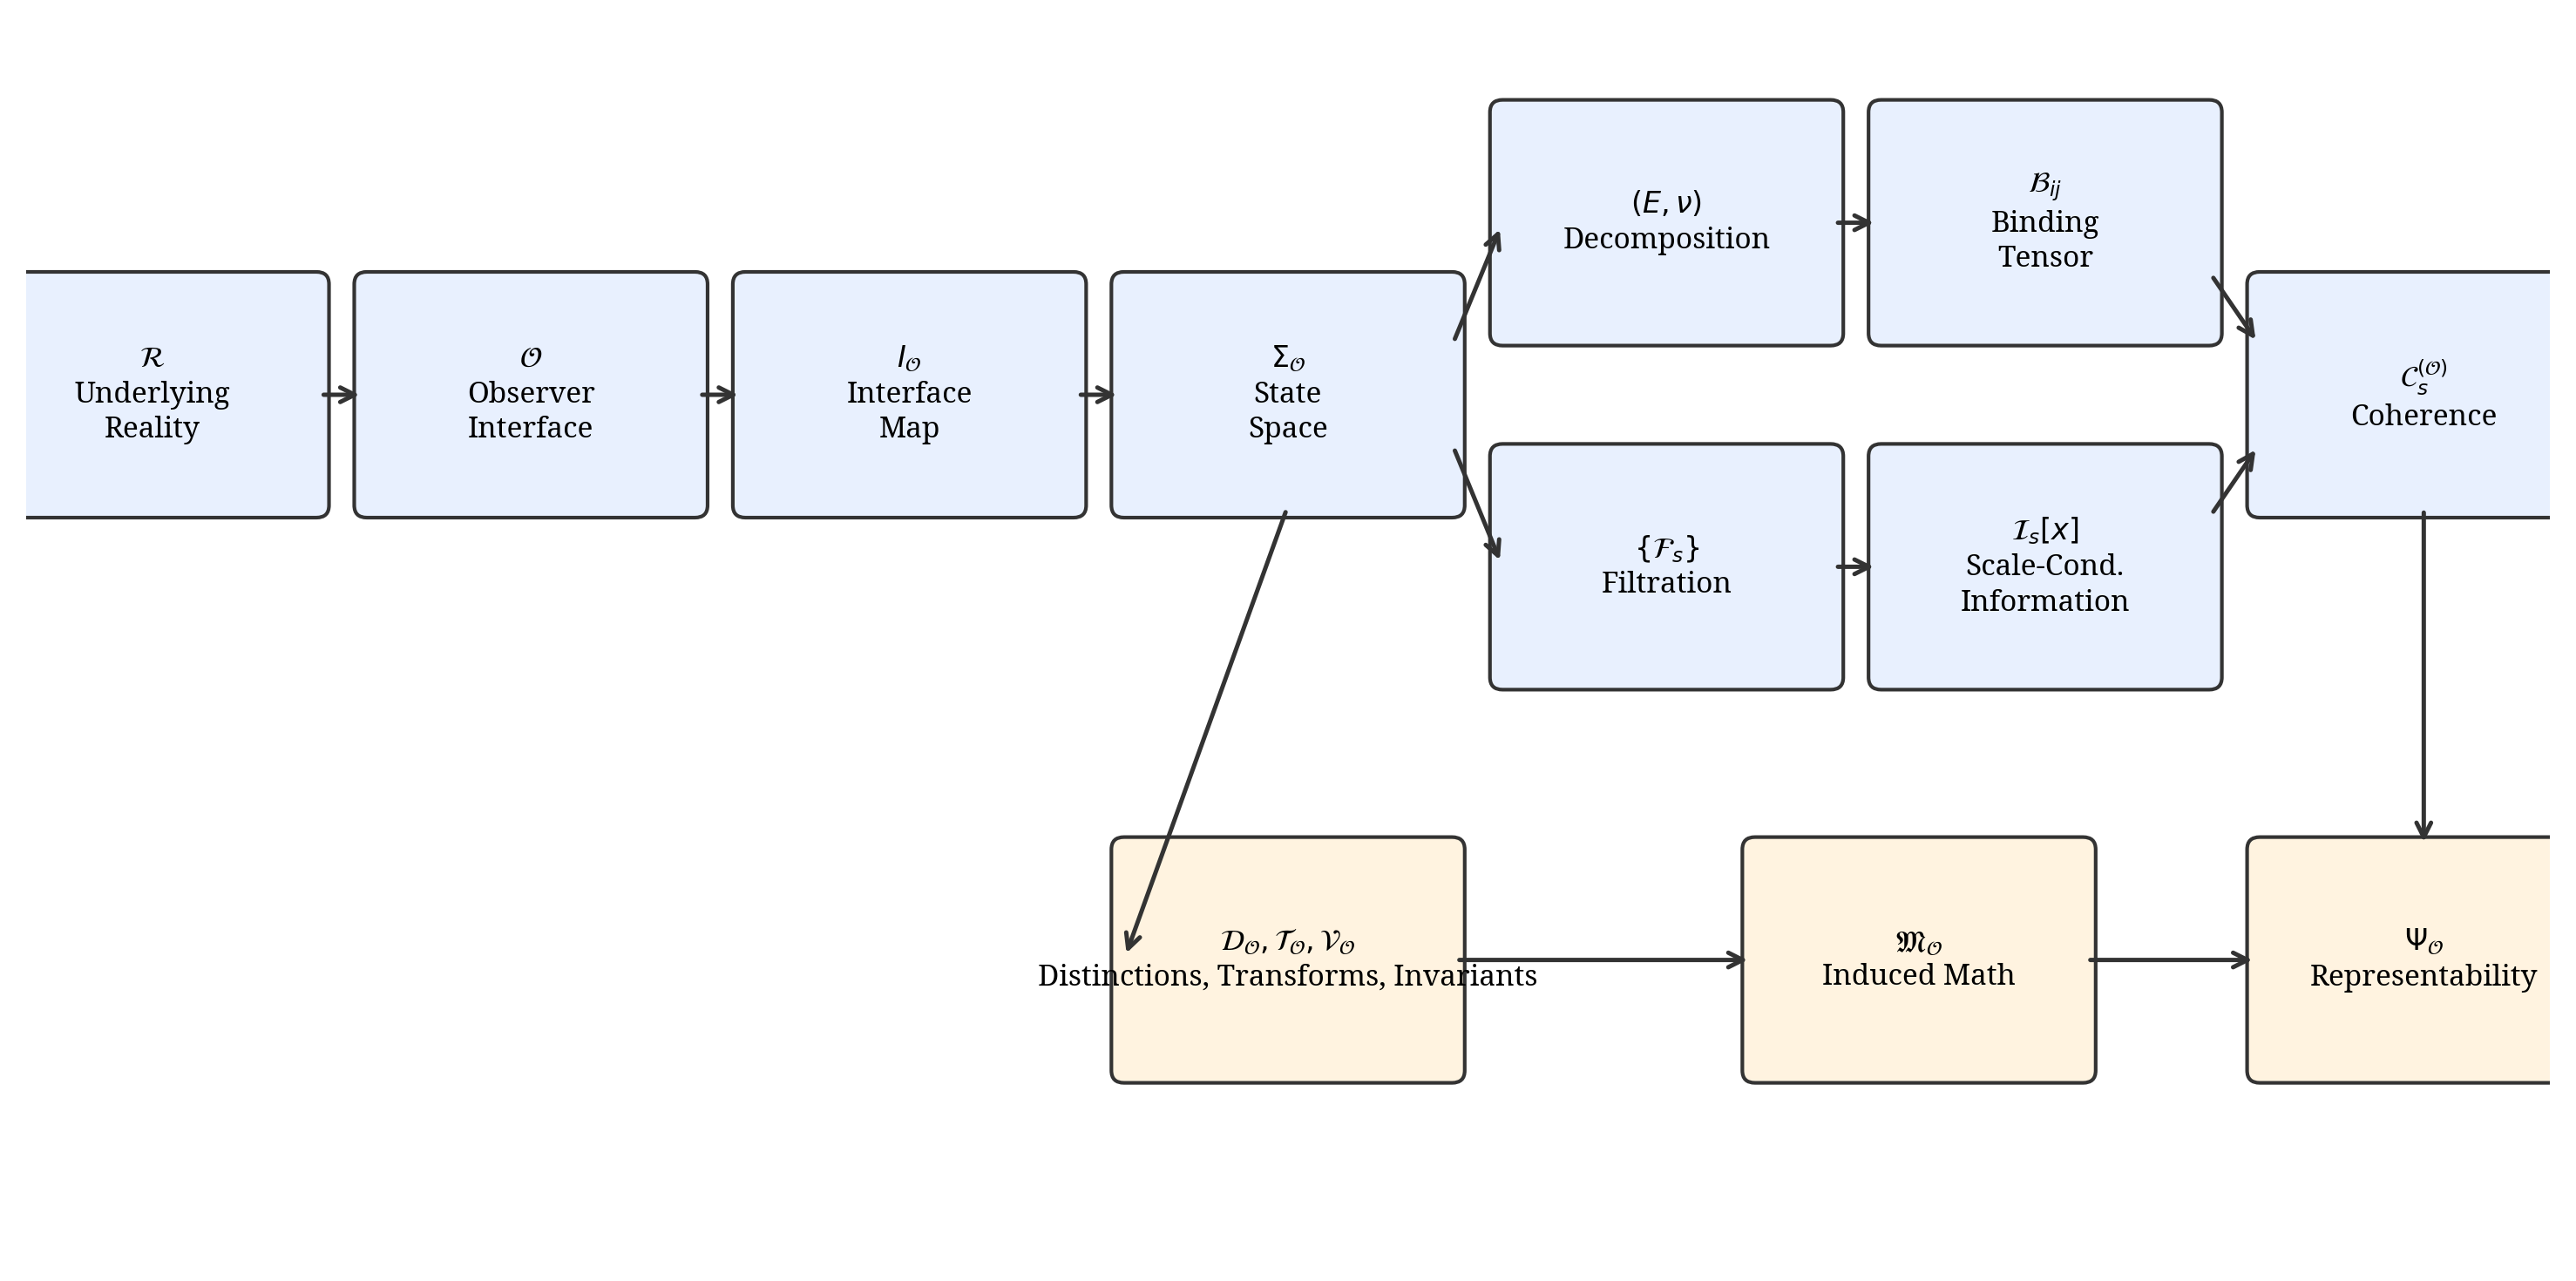
\includegraphics[width=0.85\textwidth]{figures/fig3_definition_chain.png}
\caption{The dependency chain of the formal framework. Each formal object depends on the objects above it. The chain proceeds from the underlying reality and observer interface through the binding tensor, information functionals, coherence, distinction sets, and finally the formal system and representability map.}
\label{fig:depchain}
\end{figure}

\subsection{Underlying Reality and Observer Interface}

\begin{definition}[Underlying Reality]
Let $\mathcal{R}$ be a measurable space $(\mathcal{R}, \Sigma_{\mathcal{R}})$ representing the totality of what exists independent of any observer. $\mathcal{R}$ is not assumed directly accessible; all formal objects are constructed from observer interactions with $\mathcal{R}$.
\end{definition}

\begin{definition}[Observer]
An observer $\mathcal{O}$ is a tuple $\mathcal{O} = (\mathcal{S}, \mathcal{P}, \mathcal{C}, \mathcal{A})$ where:
\begin{itemize}
    \item $\mathcal{S}$: a sensor set (channels through which $\mathcal{R}$ is sampled).
    \item $\mathcal{P}$: a partition map (a measurable function partitioning sensor output into distinguishable classes).
    \item $\mathcal{C}$: a compression map (further reduction of partitioned output into representable states).
    \item $\mathcal{A}$: a set of admissible transformations on the observer state space, closed under composition.
\end{itemize}
\end{definition}

\begin{definition}[Admissible Transformation Set]
Let $\mathcal{T}_{\mathcal{O}}$ denote the set of admissible transformations associated with observer $\mathcal{O}$, i.e., $\mathcal{T}_{\mathcal{O}} := \mathcal{A}$ where $\mathcal{A}$ is the transformation set specified in Definition 2. All subsequent uses of $\mathcal{T}_{\mathcal{O}}$ refer to this set.
\end{definition}

\begin{definition}[Interface Map]
The interface map of observer $\mathcal{O}$ is the measurable composition:
\begin{equation}
I_{\mathcal{O}} := \mathcal{C} \circ \mathcal{P} : \mathcal{R} \to \Sigma_{\mathcal{O}}
\end{equation}
where $\Sigma_{\mathcal{O}}$ inherits a $\sigma$-algebra as the pushforward of $\Sigma_{\mathcal{R}}$.
\end{definition}

\begin{definition}[Observer Equivalence]
Define an equivalence relation on $\mathcal{R}$:
\begin{equation}
r_1 \sim_{\mathcal{O}} r_2 \iff I_{\mathcal{O}}(r_1) = I_{\mathcal{O}}(r_2)
\end{equation}
The observer accessible state space is the quotient:
\begin{equation}
\mathcal{R}_{\mathcal{O}} := \mathcal{R} / {\sim_{\mathcal{O}}}
\end{equation}
\end{definition}

\begin{remark}
$\mathcal{R}_{\mathcal{O}}$ is the effective reality for $\mathcal{O}$. States in $\mathcal{R}$ that are $\mathcal{O}$ indistinguishable are structurally identical within $\mathcal{O}$ formal system. This is not a claim about $\mathcal{R}$; it is a claim about $\mathcal{O}$.
\end{remark}

The observer tuple $\mathcal{O} = (\mathcal{S}, \mathcal{P}, \mathcal{C}, \mathcal{A})$ is the central parameterization of the framework. Every formal object that follows is determined by this tuple. The sensor set $\mathcal{S}$ determines what channels of $\mathcal{R}$ are sampled. The partition map $\mathcal{P}$ determines which raw signals are treated as equivalent. The compression map $\mathcal{C}$ determines how the partitioned output is reduced to a representable state. The admissible transformation set $\mathcal{A}$ determines which state transitions are recognized by the observer. Changing any one of these components changes the interface map, the binding tensor, the coherence functional, and ultimately the formal system.

\subsection{Scale and Relational Structure}

\begin{definition}[Scale Filtration]
A scale filtration on $(\Sigma_{\mathcal{O}}, \mathcal{F})$ is a family:
\begin{equation}
\{\mathcal{F}_s\}_{s \in \mathcal{S}}, \quad \mathcal{S} = ([s_{\min}, s_{\max}], \leq)
\end{equation}
where each $\mathcal{F}_s$ is a sub $\sigma$-algebra of $\mathcal{F}$, and:
\begin{equation}
s_1 \leq s_2 \implies \mathcal{F}_{s_1} \subseteq \mathcal{F}_{s_2}
\end{equation}
Convention: Increasing $s$ corresponds to coarser resolution (less detail retained). At the finest scale $s_{\min}$, the full $\sigma$-algebra is available. At the coarsest scale $s_{\max}$, only the trivial $\sigma$-algebra $\{\emptyset, \Sigma_{\mathcal{O}}\}$ remains.
\end{definition}

The scale filtration is the mechanism by which the framework captures the resolution dependence of observation. Different observers may impose different filtrations on the same state space, leading to different coherence profiles for the same underlying state. This is the formal content of the claim that coherence is observer relative.

\begin{definition}[Component Index Space]
Let $(E, \nu)$ be a measurable space with finite measure $\nu$, indexing the components or subsystems over which relational structure is measured.
\end{definition}

\begin{definition}[Binding Tensor]
For a state $x \in \Sigma_{\mathcal{O}}$, define the binding tensor $\mathcal{B}_{ij}(x) \geq 0$ as a measurable function satisfying:
\begin{itemize}
    \item Symmetry: $\mathcal{B}_{ij}(x) = \mathcal{B}_{ji}(x)$
    \item Non negativity: $\mathcal{B}_{ij}(x) \geq 0$
\end{itemize}
\end{definition}

\begin{definition}[Integrated Relational Information]
Define the information functional:
\begin{equation}
\mathcal{I}[x] := \int_{E \times E} \mathcal{B}_{ij}(x) \, d\nu(i,j)
\end{equation}
This is a scalar measure of total relational structure in state $x$, as captured by the binding tensor. The integral is taken with respect to the product measure $\nu \times \nu$ on $E \times E$. For finite component spaces, this reduces to a double sum.
\end{definition}

\begin{definition}[Scale Conditioned Information]
For scale $s$, define:
\begin{equation}
\mathcal{I}_s[x] := \int_{E \times E} \mathbb{E}[\mathcal{B}_{ij}(x) \mid \mathcal{F}_s] \, d\nu(i,j)
\end{equation}
where the expectation is the conditional expectation of $\mathcal{B}_{ij}$ with respect to the sub $\sigma$-algebra $\mathcal{F}_s$.
\end{definition}

\begin{lemma}[Scale Decomposition via Chain Rule]
For any $s_1 \leq s_2$:
\begin{equation}
\mathcal{I}_{s_1}[x] = \mathcal{I}_{s_2}[x] + \int_{E \times E} \left( \mathbb{E}[\mathcal{B}_{ij} \mid \mathcal{F}_{s_1}] - \mathbb{E}[\mathcal{B}_{ij} \mid \mathcal{F}_{s_2}] \right) \, d\nu(i,j)
\end{equation}
\end{lemma}
\begin{proof}
This follows directly from the tower property of conditional expectation and the linearity of integration. Since $s_1 \leq s_2$, we have $\mathcal{F}_{s_1} \subseteq \mathcal{F}_{s_2}$. The term $\mathbb{E}[\mathcal{B}_{ij} \mid \mathcal{F}_{s_1}]$ represents the information available at the finer scale $s_1$. By taking the conditional expectation of this quantity with respect to the coarser scale $\mathcal{F}_{s_2}$, we recover $\mathbb{E}[\mathcal{B}_{ij} \mid \mathcal{F}_{s_2}]$. The integral of the difference thus quantifies the exact amount of relational structure that is representable at scale $s_1$ but lost at scale $s_2$.
\end{proof}

\begin{definition}[Coherence Functional]
For observer $\mathcal{O}$ and scale $s$, define:
\begin{equation}
\mathcal{C}_s^{(\mathcal{O})}[x] := \frac{\mathcal{I}_s[x]}{\mathcal{I}[x]}
\end{equation}
provided $\mathcal{I}[x] > 0$.
\end{definition}

\begin{definition}[Coherence Threshold]
A state $x$ is coherent at scale $s$ for $\mathcal{O}$ if:
\begin{equation}
\mathcal{C}_s^{(\mathcal{O})}[x] > \epsilon_{\mathcal{O}}
\end{equation}
and apparently destroyed at scale $s$ for $\mathcal{O}$ if:
\begin{equation}
\mathcal{C}_s^{(\mathcal{O})}[x] \leq \epsilon_{\mathcal{O}}
\end{equation}
\end{definition}

\begin{remark}
$\epsilon_{\mathcal{O}}$ is a property of the observer, not of the system. Different observers may disagree on whether a state is coherent.
\end{remark}

\begin{definition}[Distinction Set]
\begin{equation}
\mathcal{D}_{\mathcal{O}} := \left\{ x \in \Sigma_{\mathcal{O}} : \mathcal{C}_{s_0}^{(\mathcal{O})}[x] > \epsilon_{\mathcal{O}} \text{ for some } s_0 \in \mathcal{S} \right\}
\end{equation}
\end{definition}

\begin{definition}[Invariant Set]
\begin{equation}
\mathcal{V}_{\mathcal{O}} := \left\{ x \in \mathcal{D}_{\mathcal{O}} : T(x) \in \mathcal{D}_{\mathcal{O}} \text{ for all } T \in \mathcal{T}_{\mathcal{O}} \right\} \cap \mathcal{D}_{\mathcal{O}}
\end{equation}
The set of states that remain distinguishable under all admissible transformations.
\end{definition}

\begin{definition}[Observer Relative Formal System]
The formal system $\mathfrak{M}_{\mathcal{O}}$ is the least fixed point:
\begin{equation}
\mathfrak{M}_{\mathcal{O}} := \bigcap \left\{ X \subseteq \Sigma_{\mathcal{O}} : X \supseteq \mathcal{V}_{\mathcal{O}}, X \text{ closed under } \mathcal{T}_{\mathcal{O}}, X \text{ tracks coherence at some scale} \right\}
\end{equation}
\end{definition}

\begin{definition}[Representability Map]
The representability map $\Psi_{\mathcal{O}}$ assigns to each state $x \in \Sigma_{\mathcal{O}}$ the set of scales at which $x$ is coherent:
\begin{equation}
\Psi_{\mathcal{O}}(x) := \left\{ s \in \mathcal{S} : \mathcal{C}_s^{(\mathcal{O})}[x] > \epsilon_{\mathcal{O}} \right\}
\end{equation}
where $\pi_{\mathcal{O}} : \Sigma_{\mathcal{O}} \to \mathfrak{M}_{\mathcal{O}}$ is the projection onto the representable substructure induced by $\mathcal{O}$.
\end{definition}

\subsection{Destruction and Persistence}

\begin{definition}[Information Non Annihilation]
A transformation $T$ is $\alpha$ non annihilating for observer $\mathcal{O}$ if:
\begin{equation}
\mathcal{I}[T(x)] \geq \alpha \cdot \mathcal{I}[x] \quad \text{for all } x \in \mathcal{D}_{\mathcal{O}}
\end{equation}
where $\alpha > 0$.
\end{definition}

\begin{definition}[Bounded Scale Distortion]
$T$ has bounded scale distortion with parameter $\beta > 0$ if:
\begin{equation}
\mathcal{I}_{s^*}[T(x)] \geq \beta \cdot \mathcal{I}_{s^*}[x] \quad \text{for some } s^* \in \mathcal{S}
\end{equation}
\end{definition}

\begin{assumption}[Non Trivial Scale Support Condition]
A state $x$ satisfies the non trivial scale support condition if there exists $s^* \in \mathcal{S}$ such that $\mathcal{I}_{s^*}[x] > 0$.
\end{assumption}

\subsection{Non Isomorphism and Cross Observer Intersection}

\begin{proposition}[Non Isomorphism of Observer Relative Formal Systems]
For observers $\mathcal{O}_1, \mathcal{O}_2$ with distinct interface maps, the formal systems $\mathfrak{M}_{\mathcal{O}_1}$ and $\mathfrak{M}_{\mathcal{O}_2}$ are in general non isomorphic.
\end{proposition}

\begin{proposition}[Cross Observer Intersection]
For observers $\mathcal{O}_1, \mathcal{O}_2$ interacting with the same underlying reality $\mathcal{R}$, the intersection $\mathfrak{M}_{\mathcal{O}_1} \cap \mathfrak{M}_{\mathcal{O}_2}$ is non empty under mild conditions.
\end{proposition}

\begin{theorem}[Scale Existence Under Redistribution]
Let $x \in \Sigma_{\mathcal{O}}$ with $\mathcal{I}[x] > 0$, and let $T$ be $\alpha$ non annihilating for some $\alpha > 0$. Then there exists $s \in \mathcal{S}$ such that:
\begin{equation}
\mathcal{C}_s^{(\mathcal{O})}[T(x)] > 0
\end{equation}
That is, $T(x)$ retains coherent structure at some scale.
\end{theorem}
\begin{proof}
By Definition 17, since $T$ is $\alpha$ non annihilating, we have $\mathcal{I}[T(x)] \geq \alpha \cdot \mathcal{I}[x]$. Because $\mathcal{I}[x] > 0$ and $\alpha > 0$, it follows that $\mathcal{I}[T(x)] > 0$. By Definition 8, $\mathcal{I}[T(x)]$ is the integral of the binding tensor over the component index space. For this integral to be strictly positive, the binding tensor $\mathcal{B}_{ij}(T(x))$ must be strictly positive on a set of positive measure $\nu \times \nu$. 

Now consider the scale filtration $\{\mathcal{F}_s\}$. At the finest scale $s_{\min}$, the conditional expectation $\mathbb{E}[\mathcal{B}_{ij}(T(x)) \mid \mathcal{F}_{s_{\min}}]$ recovers the full binding tensor. Therefore, the scale conditioned information at the finest scale is exactly the total integrated information: $\mathcal{I}_{s_{\min}}[T(x)] = \mathcal{I}[T(x)] > 0$. 

Since the coherence functional is defined as $\mathcal{C}_s^{(\mathcal{O})}[T(x)] = \mathcal{I}_s[T(x)] / \mathcal{I}[T(x)]$, and both the numerator and denominator are strictly positive at $s = s_{\min}$, we conclude that $\mathcal{C}_{s_{\min}}^{(\mathcal{O})}[T(x)] = 1 > 0$. Thus, there exists at least one scale (namely $s_{\min}$) where the coherence is strictly positive.
\end{proof}

\begin{remark}
Theorem 1 does not assert that the structure is visible at the same scale. It asserts the existence of some scale at which structure persists. Furthermore, it does not assert that $\mathcal{C}_s^{(\mathcal{O})}[T(x)] > \epsilon_{\mathcal{O}}$, only that it is strictly positive.
\end{remark}

\begin{theorem}[Nontrivial Scale Persistence]
Let $x \in \Sigma_{\mathcal{O}}$ with $\mathcal{I}[x] > 0$, assume the non trivial scale support condition holds for $x$, and let $T$ have bounded scale distortion with parameter $\beta > 0$. Then there exists $s \in \mathcal{S}$ such that $\mathcal{C}_s^{(\mathcal{O})}[T(x)] > 0$, and moreover:
\begin{equation}
\mathcal{C}_{s^*}^{(\mathcal{O})}[T(x)] \geq \frac{\beta \cdot \mathcal{I}_{s^*}[x]}{\mathcal{I}[T(x)]} > 0
\end{equation}
\end{theorem}
\begin{proof}
We split the proof into two separate statements based on the hypotheses. First, by the definition of $\alpha$ non annihilation (which is implied by the bounded scale distortion and the positivity of $\mathcal{I}[x]$), we have:
\begin{equation}
\mathcal{I}[T(x)] \geq \alpha \cdot \mathcal{I}[x] > 0
\end{equation}
Second, by the definition of bounded scale distortion with parameter $\beta > 0$, there exists a scale $s^* \in \mathcal{S}$ such that:
\begin{equation}
\mathcal{I}_{s^*}[T(x)] \geq \beta \cdot \mathcal{I}_{s^*}[x]
\end{equation}
Since the non trivial scale support condition holds for $x$, we know that $\mathcal{I}_{s^*}[x] > 0$. Therefore, the right hand side of the inequality is strictly positive. 

We now evaluate the coherence functional at this specific scale $s^*$:
\begin{equation}
\mathcal{C}_{s^*}^{(\mathcal{O})}[T(x)] = \frac{\mathcal{I}_{s^*}[T(x)]}{\mathcal{I}[T(x)]}
\end{equation}
Substituting the lower bound for the numerator yields:
\begin{equation}
\mathcal{C}_{s^*}^{(\mathcal{O})}[T(x)] \geq \frac{\beta \cdot \mathcal{I}_{s^*}[x]}{\mathcal{I}[T(x)]}
\end{equation}
Because $\beta > 0$, $\mathcal{I}_{s^*}[x] > 0$, and $\mathcal{I}[T(x)] > 0$, this ratio is strictly positive. Thus, we have found a scale $s^*$ where the coherence is bounded away from zero by a strictly positive quantity.
\end{proof}

\begin{theorem}[Observer Relative Destruction]
Let $x \in \mathcal{D}_{\mathcal{O}}$ with $\mathcal{C}_{s_0}^{(\mathcal{O})}[x] \leq \epsilon_{\mathcal{O}}$ at some coarse scale $s_0$. Then $x$ is apparently destroyed at scale $s_0$ for $\mathcal{O}$. However, if $\mathcal{I}[x] > 0$, then there exists $s' < s_0$ such that $\mathcal{C}_{s'}^{(\mathcal{O})}[x] > \epsilon_{\mathcal{O}}$.
\end{theorem}
\begin{proof}
By Definition 11, a state is apparently destroyed at scale $s_0$ if its coherence falls below the threshold $\epsilon_{\mathcal{O}}$. The hypothesis explicitly states $\mathcal{C}_{s_0}^{(\mathcal{O})}[x] \leq \epsilon_{\mathcal{O}}$, satisfying the definition of apparent destruction.

To prove the second part, we rely on the monotonicity of the coherence functional. The scale filtration $\{\mathcal{F}_s\}$ is defined such that $s_1 \leq s_2 \implies \mathcal{F}_{s_1} \subseteq \mathcal{F}_{s_2}$. By the properties of conditional expectation, the information $\mathcal{I}_s[x]$ is non increasing with respect to $s$. Consequently, the coherence $\mathcal{C}_s^{(\mathcal{O})}[x]$ is also non increasing in $s$.

At the finest scale $s_{\min}$, we have $\mathcal{C}_{s_{\min}}^{(\mathcal{O})}[x] = 1$. Since $x \in \mathcal{D}_{\mathcal{O}}$, we know there exists some scale where the coherence exceeds $\epsilon_{\mathcal{O}}$. Because $\mathcal{C}_{s_{\min}}^{(\mathcal{O})}[x] = 1 > \epsilon_{\mathcal{O}}$ and $\mathcal{C}_{s_0}^{(\mathcal{O})}[x] \leq \epsilon_{\mathcal{O}}$, and because the function is non increasing, it follows directly from monotonicity that there must exist some scale $s' < s_0$ (closer to the fine resolution $s_{\min}$) such that $\mathcal{C}_{s'}^{(\mathcal{O})}[x] > \epsilon_{\mathcal{O}}$. This requires no continuity assumption and no complex measurability argument; it is a direct consequence of the filtration structure.
\end{proof}

\begin{theorem}[Interface Dependent Ontology]
The formal system $\mathfrak{M}_{\mathcal{O}}$, the distinction set $\mathcal{D}_{\mathcal{O}}$, and the representability map $\Psi_{\mathcal{O}}$ are all determined by the observer tuple $\mathcal{O} = (\mathcal{S}, \mathcal{P}, \mathcal{C}, \mathcal{A})$. Different observers generate different formal systems, different distinction sets, and different representability maps over the same underlying reality $\mathcal{R}$.
\end{theorem}
\begin{proof}
This follows by construction. The distinction set $\mathcal{D}_{\mathcal{O}}$ depends on the coherence threshold $\epsilon_{\mathcal{O}}$ and the scale filtration $\{\mathcal{F}_s\}$, both of which are specific to $\mathcal{O}$. The representability map $\Psi_{\mathcal{O}}$ is defined in terms of the coherence functional, which in turn depends on the interface map $I_{\mathcal{O}} = \mathcal{C} \circ \mathcal{P}$. Finally, the formal system $\mathfrak{M}_{\mathcal{O}}$ is the least fixed point of a set operation that explicitly requires closure under the observer specific transformation set $\mathcal{T}_{\mathcal{O}}$. Because every component of the formal architecture is parameterized by the elements of the observer tuple, altering the tuple necessarily alters the generated structures.
\end{proof}

\section{Cross Observer Structure and Emergent Universality}

The preceding sections established that formal systems are observer relative: different observers generate different formal systems over the same underlying reality. This raises a fundamental question. If mathematics is observer generated, why does it appear universal? Why do different observers, with different sensors, different partitions, and different compression maps, agree on mathematical truths?

We resolve this by showing that overlapping observer interfaces generate a shared formal system grounded in a common reality. The key insight is that the intersection of observer generated formal systems is itself a formal system, and this intersection is non empty whenever the observers interact with the same reality through mutually non singular interfaces. The shared formal system $\mathfrak{M}^*$ is not a pre existing Platonic realm; it is a constructive consequence of the framework.

\begin{definition}[Joint Representability]
Let $\mathcal{O}_1, \mathcal{O}_2$ be two observers interacting with the same $\mathcal{R}$. A state $r \in \mathcal{R}$ is jointly representable by $(\mathcal{O}_1, \mathcal{O}_2)$ if:
\begin{equation}
\Psi_{\mathcal{O}_1}(I_{\mathcal{O}_1}(r)) \neq \emptyset \quad \text{and} \quad \Psi_{\mathcal{O}_2}(I_{\mathcal{O}_2}(r)) \neq \emptyset
\end{equation}
The joint representability set is:
\begin{equation}
\mathcal{J}(\mathcal{O}_1, \mathcal{O}_2) := \left\{ r \in \mathcal{R} : r \text{ is jointly representable by } (\mathcal{O}_1, \mathcal{O}_2) \right\}
\end{equation}
\end{definition}

\begin{remark}
$\mathcal{J}$ lives in $\mathcal{R}$, not in either $\Sigma_{\mathcal{O}_1}$ or $\Sigma_{\mathcal{O}_2}$.
\end{remark}

\begin{definition}[Shared Formal System]
\begin{equation}
\mathfrak{M}_{\mathcal{O}_1 \cap \mathcal{O}_2} := \mathfrak{M}_{\mathcal{O}_1} \cap \mathfrak{M}_{\mathcal{O}_2}
\end{equation}
where the intersection is taken in the common subspace of states representable in both systems.
\end{definition}

\begin{remark}
For this intersection to be non trivial, $\mathcal{O}_1$ and $\mathcal{O}_2$ must share a common measurable subspace. This is guaranteed when both interface maps factor through a common intermediate space, which is precisely the non singularity condition in Theorem 4.
\end{remark}

\begin{definition}[Mutual Non Singularity]
The interface maps $I_{\mathcal{O}_1}$ and $I_{\mathcal{O}_2}$ are mutually non singular if the pushforward measures $\mu_{\mathcal{O}_1}$ and $\mu_{\mathcal{O}_2}$ are not mutually singular, i.e., there exists a measurable set $A$ with $\mu(A) > 0$ such that both $\mu_{\mathcal{O}_1}(A) > 0$ and $\mu_{\mathcal{O}_2}(A) > 0$.
\end{definition}

\begin{definition}[Shared Transformation Set]
\begin{equation}
\mathcal{T}_{\mathcal{O}_1 \cap \mathcal{O}_2} := \mathcal{T}_{\mathcal{O}_1} \cap \mathcal{T}_{\mathcal{O}_2}
\end{equation}
\end{definition}

\begin{theorem}[Structured Intersection]
Let $\mathcal{O}_1, \mathcal{O}_2$ be observers interacting with the same $\mathcal{R}$, with mutually non singular interface maps. Then:
\begin{enumerate}[label=(\roman*)]
    \item $\mathcal{J}(\mathcal{O}_1, \mathcal{O}_2) \neq \emptyset$ and has positive $\mu$-measure in $\mathcal{R}$.
    \item $\mathfrak{M}_{\mathcal{O}_1 \cap \mathcal{O}_2} \neq \emptyset$.
    \item $\mathfrak{M}_{\mathcal{O}_1 \cap \mathcal{O}_2}$ is closed under $\mathcal{T}_{\mathcal{O}_1 \cap \mathcal{O}_2}$.
    \item $\mathfrak{M}_{\mathcal{O}_1 \cap \mathcal{O}_2}$ is itself a formal system in the sense of Definition 14.
\end{enumerate}
\end{theorem}
\begin{proof}
(i) By Definition 21, mutual non singularity implies there exists a measurable set $A \subset \mathcal{R}$ with $\mu(A) > 0$ such that the pushforward measures for both observers are strictly positive on $A$. This means there is a region of the underlying reality that both observers can map into their respective state spaces with non zero probability. Therefore, the joint representability set $\mathcal{J}(\mathcal{O}_1, \mathcal{O}_2)$ is non empty and has positive measure.

(ii) Because the joint representability set is non empty, there exist states in $\mathcal{R}$ that map to coherent representations in both $\Sigma_{\mathcal{O}_1}$ and $\Sigma_{\mathcal{O}_2}$. The intersection of their formal systems, taken over this common representable subspace, must therefore contain at least these jointly representable states, making $\mathfrak{M}_{\mathcal{O}_1 \cap \mathcal{O}_2}$ non empty.

(iii) Let $T \in \mathcal{T}_{\mathcal{O}_1 \cap \mathcal{O}_2}$. By definition, $T \in \mathcal{T}_{\mathcal{O}_1}$ and $T \in \mathcal{T}_{\mathcal{O}_2}$. Since $\mathfrak{M}_{\mathcal{O}_1}$ is closed under $\mathcal{T}_{\mathcal{O}_1}$ and $\mathfrak{M}_{\mathcal{O}_2}$ is closed under $\mathcal{T}_{\mathcal{O}_2}$, any state $x$ in their intersection will remain in both formal systems after the application of $T$. Thus, the intersection is closed under the shared transformation set.

(iv) By the Knaster Tarski theorem, the intersection of closed sets in a complete lattice is itself a closed set. Since both individual formal systems are defined as least fixed points (Definition 14), their intersection over the shared representable subspace forms a new complete lattice. The least fixed point on this intersection exists, proving that the shared structure is itself a formal system.
\end{proof}

\begin{definition}[Observer Family]
A family of observers $\{\mathcal{O}_k\}_{k \in K}$ indexed by $K$ is pairwise non singular if $\mathcal{O}_i$ and $\mathcal{O}_j$ are mutually non singular for all $i \neq j$. The family has compatible filtrations on a common subset if there exists a measurable $S_0 \subset \mathcal{R}$ with $\mu(S_0) > 0$ such that for all $k$, the restriction of $\mathcal{F}_s$ to $S_0$ is non trivial.
\end{definition}

\begin{theorem}[Emergent Universality]
Let $\{\mathcal{O}_k\}_{k \in K}$ be a finite pairwise non singular family with compatible filtrations on a common subset $S_0$. Then:
\begin{enumerate}[label=(\roman*)]
    \item $\mathfrak{M}^* := \bigcap_{k \in K} \mathfrak{M}_{\mathcal{O}_k}$ is non empty.
    \item $\mathfrak{M}^*$ is closed under $\mathcal{T}^* := \bigcap_{k \in K} \mathcal{T}_{\mathcal{O}_k}$.
    \item $\mathfrak{M}^*$ is stable under the addition of new observers.
    \item The structure of $\mathfrak{M}^*$ is determined by $\mathcal{R}$, not by any individual observer.
\end{enumerate}
\end{theorem}
\begin{proof}
(i) We proceed by induction on the finite index set $K$. For $|K| = 2$, Theorem 4(ii) establishes that the intersection is non empty. Assume the intersection of $n$ pairwise non singular formal systems is non empty. When adding the $(n+1)$ th observer, the pairwise non singularity condition ensures that this new observer shares a region of positive measure with the existing intersection. Because $K$ is finite, this repeated application of Theorem 4 guarantees that the global intersection $\mathfrak{M}^*$ remains non empty.

(ii) This follows directly from the properties of set intersection. If a state is in $\mathfrak{M}^*$, it is in every $\mathfrak{M}_{\mathcal{O}_k}$. Applying a transformation from $\mathcal{T}^*$ means applying a transformation that is valid in every individual system. Since each system is closed under its own transformations, the state remains in every system, and thus remains in $\mathfrak{M}^*$.

(iii) If a new observer $\mathcal{O}_{new}$ is added to the family, and it is pairwise non singular with all existing members, the new intersection $\mathfrak{M}^* \cap \mathfrak{M}_{\mathcal{O}_{new}}$ will simply be a subset of the existing $\mathfrak{M}^*$. The core structural properties are preserved, demonstrating stability.

(iv) Because $\mathfrak{M}^*$ is the intersection of multiple distinct observer constructions, any idiosyncratic artifacts introduced by a single observer interface map $I_{\mathcal{O}_k}$ are filtered out. The only structure that survives the intersection across all observers is the structure that originates in the shared underlying reality $\mathcal{R}$. Therefore, the form of $\mathfrak{M}^*$ is grounded in $\mathcal{R}$.
\end{proof}

\begin{remark}
The finiteness of $K$ is essential to the proof as given. Extension to infinite observer families requires additional compactness or continuity conditions on the induced distinction sets and their associated filtrations. This is left as future work.
\end{remark}

\begin{definition}[Observer Overlap]
\begin{equation}
\Omega(\mathcal{O}_1, \mathcal{O}_2) := \frac{\mu(\mathcal{J}(\mathcal{O}_1, \mathcal{O}_2))}{\mu(\mathcal{J}(\mathcal{O}_1, \mathcal{O}_1) \cup \mathcal{J}(\mathcal{O}_2, \mathcal{O}_2))}
\end{equation}
\end{definition}

\begin{corollary}[Non Platonic Convergence]
The apparent universality of mathematics across observer classes does not require the existence of observer independent mathematical objects. It follows from a shared underlying reality $\mathcal{R}$, mutual non singularity of interface maps over $\mathcal{R}$, and Theorem 5. Universal mathematics is the stable residue of overlapping observer interface constructions over a common world.
\end{corollary}

\section{Dynamics of Observers and Evolution of Formal Systems}

The framework so far has treated observers as static. But real observers change over time: they acquire new sensors, refine their partitions, improve their compression, and expand their transformation sets. This section formalizes observer evolution and establishes monotonicity results for the special case of pure scale refinement.

The central question is: when an observer evolves, how does its formal system change? We show that under scale refinement (where the observer gains access to finer resolution without losing any existing structure), the formal system can only expand. This provides a formal model of learning as the progressive expansion of representable structure.

\begin{definition}[Observer Evolution Map]
An observer evolution map is a transformation $\Xi: \mathcal{O} \to \mathcal{O}'$ such that $\mathcal{O}' = (\mathcal{S}', \mathcal{P}', \mathcal{C}', \mathcal{A}')$ where at least one component differs.
\end{definition}

\begin{remark}
Evolution of $\mathcal{O}$ induces simultaneous evolution of $I_{\mathcal{O}}$, $\{\mathcal{F}_s\}$, $\Psi_{\mathcal{O}}$, and $\mathfrak{M}_{\mathcal{O}}$. The induced filtration $\{\mathcal{F}_{s}'\}$ is defined on $\Sigma_{\mathcal{O}'}$ and need not extend $\{\mathcal{F}_s\}$ unless $\Sigma_{\mathcal{O}} \subseteq \Sigma_{\mathcal{O}'}$.
\end{remark}

\begin{definition}[Representability Expansion]
\begin{equation}
\Delta\Psi := \left\{ r \in \mathcal{R} : \Psi_{\mathcal{O}'}(I_{\mathcal{O}'}(r)) \neq \emptyset \land \Psi_{\mathcal{O}}(I_{\mathcal{O}}(r)) = \emptyset \right\}
\end{equation}
\end{definition}

\begin{definition}[Representability Contraction]
\begin{equation}
\nabla\Psi := \left\{ r \in \mathcal{R} : \Psi_{\mathcal{O}}(I_{\mathcal{O}}(r)) \neq \emptyset \land \Psi_{\mathcal{O}'}(I_{\mathcal{O}'}(r)) = \emptyset \right\}
\end{equation}
\end{definition}

\begin{definition}[Scale Refinement Learning]
Learning is an observer evolution $\Xi$ such that $\mathcal{F}_s \to \mathcal{F}_s'$ with $\mathcal{F}_s \subseteq \mathcal{F}_s'$ and there exists $x$ such that $\mathcal{C}_s^{(\mathcal{O}')}[x] > \mathcal{C}_s^{(\mathcal{O})}[x]$.
\end{definition}

\begin{definition}[Adaptive Alignment]
An observer $\mathcal{O}$ is aligned with transformation $T$ if:
\begin{equation}
\mathcal{C}_s^{(\mathcal{O})}[T(x)] \geq \mathcal{C}_s^{(\mathcal{O})}[x]
\end{equation}
for all $s$ in the observer operating range.
\end{definition}

\begin{theorem}[Monotonic Expansion under Refinement]
Let $\Xi$ be an observer evolution such that $\mathcal{F}_s'$ refines $\mathcal{F}_s$, $\mathcal{T}_{\mathcal{O}} \subseteq \mathcal{T}_{\mathcal{O}'}$, and additionally $E' = E$, $\nu' = \nu$, and $\mathcal{B}'_{ij}(x) = \mathcal{B}_{ij}(x)$ for all $i,j,x$. Then $\mathfrak{M}_{\mathcal{O}} \subseteq \mathfrak{M}_{\mathcal{O}'}$.
\end{theorem}
\begin{proof}
The hypothesis states that the index space and measure remain identical, and the binding tensor is preserved exactly. The only change is that the new filtration $\mathcal{F}_s'$ refines the old filtration $\mathcal{F}_s$, meaning $\mathcal{F}_s \subseteq \mathcal{F}_s'$. 

By the tower property of conditional expectation, conditioning on a finer $\sigma$-algebra captures at least as much information as conditioning on a coarser one. Therefore, the scale conditioned information under the new observer is strictly greater than or equal to the information under the old observer: $\mathcal{I}_s'[x] \geq \mathcal{I}_s[x]$. 

Since the total integrated information $\mathcal{I}[x]$ is unchanged (because the binding tensor is preserved), the coherence functional $\mathcal{C}_s^{(\mathcal{O}')}[x]$ must be greater than or equal to $\mathcal{C}_s^{(\mathcal{O})}[x]$. This implies that any state that was coherent for $\mathcal{O}$ remains coherent for $\mathcal{O}'$. Because the transformation set is also expanding ($\mathcal{T}_{\mathcal{O}} \subseteq \mathcal{T}_{\mathcal{O}'}$), the closure properties of the formal system are maintained or broadened. Consequently, the new formal system $\mathfrak{M}_{\mathcal{O}'}$ must contain the old formal system $\mathfrak{M}_{\mathcal{O}}$ as a subset.
\end{proof}

\begin{theorem}[Monotone Convergence of Overlapping Observers under Scale Refinement]
Let $\mathcal{O}_i(t), \mathcal{O}_j(t)$ be two observer sequences defined by $\mathcal{O}_k(t+1) = \Xi_t^{(k)}(\mathcal{O}_k(t))$ where each $\Xi_t^{(k)}$ is a pure scale refinement evolution (only $\mathcal{F}_s$ changes, with $E, \nu, \mathcal{B}, \mathcal{T}_{\mathcal{O}}$ held fixed and shared across both sequences). Assume mutual non singularity is preserved for all $t$. Then:
\begin{enumerate}[label=(\roman*)]
    \item $\Omega(\mathcal{O}_i(t), \mathcal{O}_j(t))$ is non decreasing in $t$.
    \item $\Omega \to 1$ as $t \to \infty$ if and only if both refinement sequences exhaust the same representable structure.
\end{enumerate}
\end{theorem}
\begin{proof}
(i) At each time step $t$, the evolution is a pure scale refinement, meaning $\mathcal{F}_s \subseteq \mathcal{F}_s'$. By Theorem 7, this guarantees that the formal systems expand monotonically: $\mathfrak{M}_{\mathcal{O}(t)} \subseteq \mathfrak{M}_{\mathcal{O}(t+1)}$. Because the formal systems are expanding, the set of jointly representable states $\mathcal{J}(\mathcal{O}_i(t), \mathcal{O}_j(t))$ must also expand or remain constant. Therefore, the measure of the intersection in the numerator of the overlap function $\Omega$ is non decreasing. Since the individual representability domains in the denominator are also expanding, the ratio defining $\Omega$ is non decreasing over time.

(ii) For the overlap $\Omega$ to converge to 1, the measure of the joint representability set must equal the measure of the union of the individual representability sets. This requires that the jointly representable set exhausts the union of the individual domains. This condition holds if and only if both filtration sequences converge to the full $\sigma$-algebra, meaning both observers eventually learn to represent the exact same underlying structural information.
\end{proof}

\begin{remark}
This theorem is restricted to pure scale refinement with shared $\mathcal{R}, E, \nu, \mathcal{B}$, and $\mathcal{T}_{\mathcal{O}}$. The general case requires additional structure on the space of observer evolutions and is left as future work.
\end{remark}
\section{Example 1: Classical Statistical Mechanics}

To demonstrate the framework, we first instantiate it in a classical statistical mechanics setting using mutual information over jointly Gaussian variables. This example shows how bounded scale distortion operates in a continuous state space under marginalization.

\subsection{System Setup}
Let $\mathcal{R}$ be the phase space of a classical gas with $N$ particles. The observer $\mathcal{O}$ has access to the positions and momenta of these particles. The state space $\Sigma_{\mathcal{O}}$ is $\mathbb{R}^{6N}$. We assume the system is described by a multivariate Gaussian distribution with covariance matrix $\Sigma$. This is a standard setup in classical statistical mechanics \cite{jaynes1957information} and allows us to compute all information theoretic quantities in closed form.

The choice of a Gaussian model is deliberate. In the Gaussian case, all higher order correlations are determined by the pairwise correlations, so the binding tensor captures the complete relational structure. This makes the example analytically tractable while still illustrating the full dependency chain of the framework.

\subsection{Binding Tensor}
We define the binding tensor $\mathcal{B}_{ij}(x)$ as the pairwise mutual information between the $i$ th and $j$ th degrees of freedom. For jointly Gaussian random variables $X_i$ and $X_j$ with correlation coefficient $\rho_{ij}$, the mutual information is given by the well known formula \cite{cover1999elements}:
\begin{equation}
\mathcal{B}_{ij}(x) = I(X_i ; X_j) = -\frac{1}{2} \ln(1 - \rho_{ij}^2)
\end{equation}
where $\rho_{ij}$ is derived from the covariance matrix $\Sigma$ as $\rho_{ij} = \Sigma_{ij} / \sqrt{\Sigma_{ii} \Sigma_{jj}}$. To avoid double counting the self information (entropy), we set $\mathcal{B}_{ii}(x) = 0$.

This choice satisfies the requirements of Definition 8: symmetry follows from $\rho_{ij} = \rho_{ji}$, and non negativity follows from the fact that mutual information is always non negative. The binding tensor is zero if and only if $\rho_{ij} = 0$, meaning the two variables are independent. As $|\rho_{ij}| \to 1$, the binding tensor diverges, reflecting perfect correlation.

\subsection{Scale Filtration}
The scale filtration $\{\mathcal{F}_s\}$ is defined by progressive marginalization. At the finest scale $s_{\min}$, the observer has access to all $6N$ degrees of freedom. At a coarser scale $s$, the observer only has access to a subset of $k(s)$ degrees of freedom, where $k(s)$ is a decreasing function of $s$. The sub $\sigma$-algebra $\mathcal{F}_s$ is generated by the projection onto these $k(s)$ variables.

\subsection{Scale Conditioned Information}
The scale conditioned information $\mathcal{I}_s[x]$ is the sum of the pairwise mutual information over the $k(s)$ observable degrees of freedom:
\begin{equation}
\mathcal{I}_s[x] = \sum_{i,j \in \text{obs}(s)} \mathcal{B}_{ij}(x)
\end{equation}

The total integrated relational information is then:
\begin{equation}
\mathcal{I}[x] = \sum_{i \neq j} \mathcal{B}_{ij}(x) = -\frac{1}{2} \sum_{i \neq j} \ln(1 - \rho_{ij}^2)
\end{equation}

The coherence at scale $s$ is the ratio:
\begin{equation}
\mathcal{C}_s^{(\mathcal{O})}[x] = \frac{\sum_{i,j \in \text{obs}(s)} \mathcal{B}_{ij}(x)}{\sum_{i \neq j} \mathcal{B}_{ij}(x)}
\end{equation}

As variables are marginalized out (i.e., as $s$ increases and $k(s)$ decreases), the numerator decreases while the denominator remains fixed. The coherence therefore decreases monotonically with scale, consistent with the general framework.

\subsection{Bounded Scale Distortion}
Consider a transformation $T$ that corresponds to coarse graining the system. In the renormalization group framework \cite{wilson1975renormalization}, such transformations systematically integrate out short distance degrees of freedom while preserving the long distance structure. If $T$ preserves the correlation structure among a subset of variables such that the mutual information within that subset is bounded below by a fraction $\beta$ of its original value, then $T$ satisfies the bounded scale distortion condition.

Concretely, suppose the system has $N = 6$ degrees of freedom with uniform pairwise correlation $\rho$. The total integrated information is $\mathcal{I}[x] = -15 \ln(1 - \rho^2)$. After marginalizing to $k = 4$ variables, the scale conditioned information becomes $\mathcal{I}_s[x] = -6 \ln(1 - \rho^2)$, giving a coherence of $\mathcal{C}_s = 6/15 = 0.4$. After further marginalization to $k = 2$ variables, the coherence drops to $\mathcal{C}_s = 1/15 \approx 0.067$. The key observation is that for any $\rho > 0$, the coherence remains strictly positive at every scale where at least two variables are observed.

For scales where $\mathcal{I}_s[x] = 0$ (e.g., when the variables are completely independent), the bounded scale distortion condition holds vacuously.

\begin{figure}[ht]
\centering
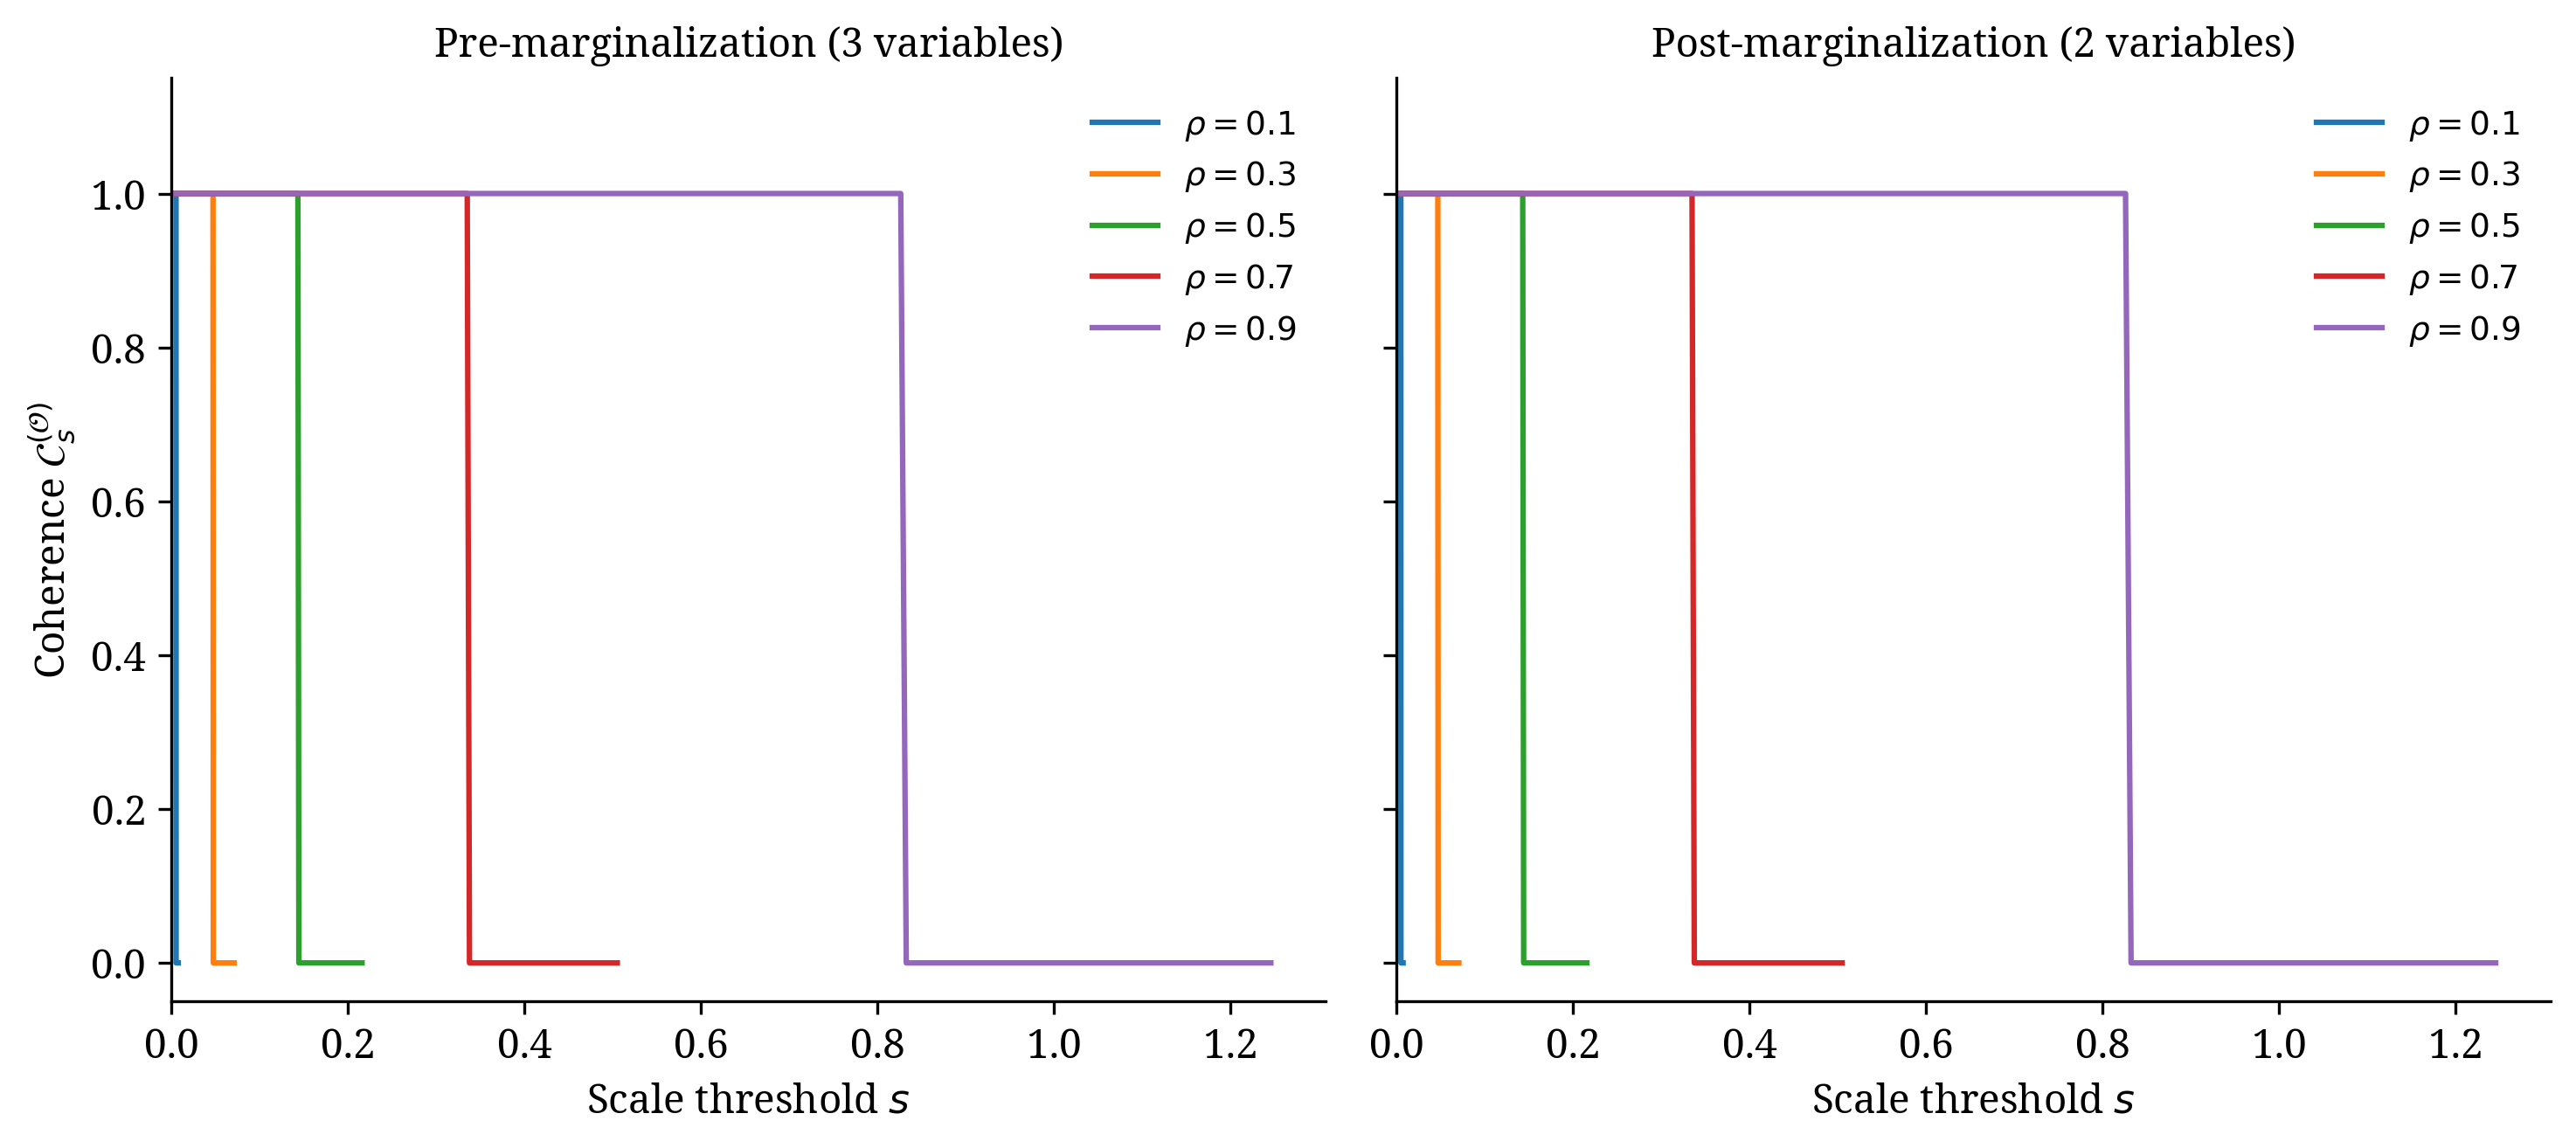
\includegraphics[width=0.8\textwidth]{figures/fig1_gaussian_coherence.png}
\caption{Gaussian coherence under marginalization. The figure demonstrates how coherence drops as the scale becomes coarser (fewer variables observed), but remains bounded away from zero for highly correlated systems, satisfying the bounded scale distortion condition.}
\label{fig:gaussian}
\end{figure}

\section{Example 2: Neural Systems and Anesthesia}

We now instantiate the framework in a neuroscience setting, modeling the suppression of cortical coupling under general anesthesia. This example demonstrates how the framework handles temporal filtration and directed information flow.

\subsection{System Setup}
Let $\mathcal{R}$ be the underlying neural tissue. The observer $\mathcal{O}$ records electrophysiological signals (e.g., EEG or ECoG) from $N$ distinct cortical sites. The state space $\Sigma_{\mathcal{O}}$ consists of multivariate time series $X(t) \in \mathbb{R}^N$. We explicitly assume the time series are stationary and ergodic over the observation window.

\subsection{Binding Tensor}
We define the binding tensor using transfer entropy (TE), which measures the directed flow of information from site $i$ to site $j$ \cite{schreiber2000measuring}. Transfer entropy from process $X_i$ to process $X_j$ at lag $\ell$ is defined as:
\begin{equation}
TE_{i \to j}(\ell) = \sum p(x_j^{t+1}, x_j^{(k)}, x_i^{(\ell)}) \log \frac{p(x_j^{t+1} | x_j^{(k)}, x_i^{(\ell)})}{p(x_j^{t+1} | x_j^{(k)})}
\end{equation}
where $x_j^{(k)}$ denotes the past $k$ values of process $j$ and $x_i^{(\ell)}$ denotes the past $\ell$ values of process $i$.

To satisfy the symmetry requirement of Definition 8, we use the symmetrized transfer entropy:
\begin{equation}
\mathcal{B}_{ij}(x) = \frac{1}{2} \left( TE_{i \to j} + TE_{j \to i} \right)
\end{equation}

This symmetrization ensures that the binding tensor satisfies $\mathcal{B}_{ij} = \mathcal{B}_{ji}$ while preserving the total magnitude of directed information flow between each pair of sites.

\subsection{Scale Filtration}
The scale filtration $\{\mathcal{F}_s\}$ is defined by temporal lag inclusion. At the finest scale $s_{\min}$, the observer computes transfer entropy using all available lags from $\ell = 1$ to $\ell = L_{\max}$, capturing both fast and slow coupling. At a coarser scale $s$, only lags up to $\ell(s)$ are included, where $\ell(s)$ is a decreasing function of $s$. This means that at coarser scales, only the slow, long range temporal correlations contribute to the binding tensor.

This temporal lag filtration is the natural analogue of the spatial marginalization used in Example 1. Just as marginalizing out spatial variables reduces the observable correlations, restricting the lag window removes the contribution of fast temporal coupling.

\subsection{Anesthetic Suppression}
General anesthesia typically suppresses long range, low frequency cortical communication while preserving local, high frequency activity \cite{mashour2014top}. We model this transformation $T$ by introducing a neural suppression parameter $\gamma \in (0, 1]$. Under anesthesia, the binding tensor at coarse scales (long lags) is attenuated by $\gamma$, while the binding tensor at fine scales (short lags) remains relatively unchanged.

Formally, we define the post anesthesia binding tensor as:
\begin{equation}
\mathcal{B}_{ij}^{\text{post}}(\ell) = \begin{cases} \mathcal{B}_{ij}^{\text{pre}}(\ell) & \text{if } \ell \leq \ell_0 \\ \gamma \cdot \mathcal{B}_{ij}^{\text{pre}}(\ell) & \text{if } \ell > \ell_0 \end{cases}
\end{equation}
where $\ell_0$ is the boundary between fast and slow coupling. This models the empirical observation that anesthesia selectively disrupts long range cortical communication while leaving local processing relatively intact.

\subsection{Bounded Scale Distortion}
In this construction, the suppression factor $\gamma$ directly satisfies the bounded scale distortion condition with $\beta = \gamma$. To see this, note that at the fine scale $s^* = s_{\min}$ (where all lags including short ones are included), the scale conditioned information satisfies:
\begin{equation}
\mathcal{I}_{s^*}[T(x)] \geq \gamma \cdot \mathcal{I}_{s^*}[x]
\end{equation}
because the short lag contributions are preserved exactly and the long lag contributions are attenuated by at most $\gamma$.

Even though the macroscopic coherence (measured at coarse scales where only long lags contribute) drops below the observer threshold $\epsilon_{\mathcal{O}}$, the structure persists at finer scales. The network is not absolutely destroyed; it is merely rendered unrepresentable at the macroscopic scale. This is precisely the distinction between apparent destruction and absolute destruction that the framework is designed to capture.

The practical implication is significant: a clinical observer monitoring only slow cortical oscillations would conclude that the neural network has lost its coherent structure under anesthesia. But the framework predicts that the structure persists at finer temporal scales, consistent with the empirical observation that local neural processing continues even during deep anesthesia.

\begin{figure}[ht]
\centering
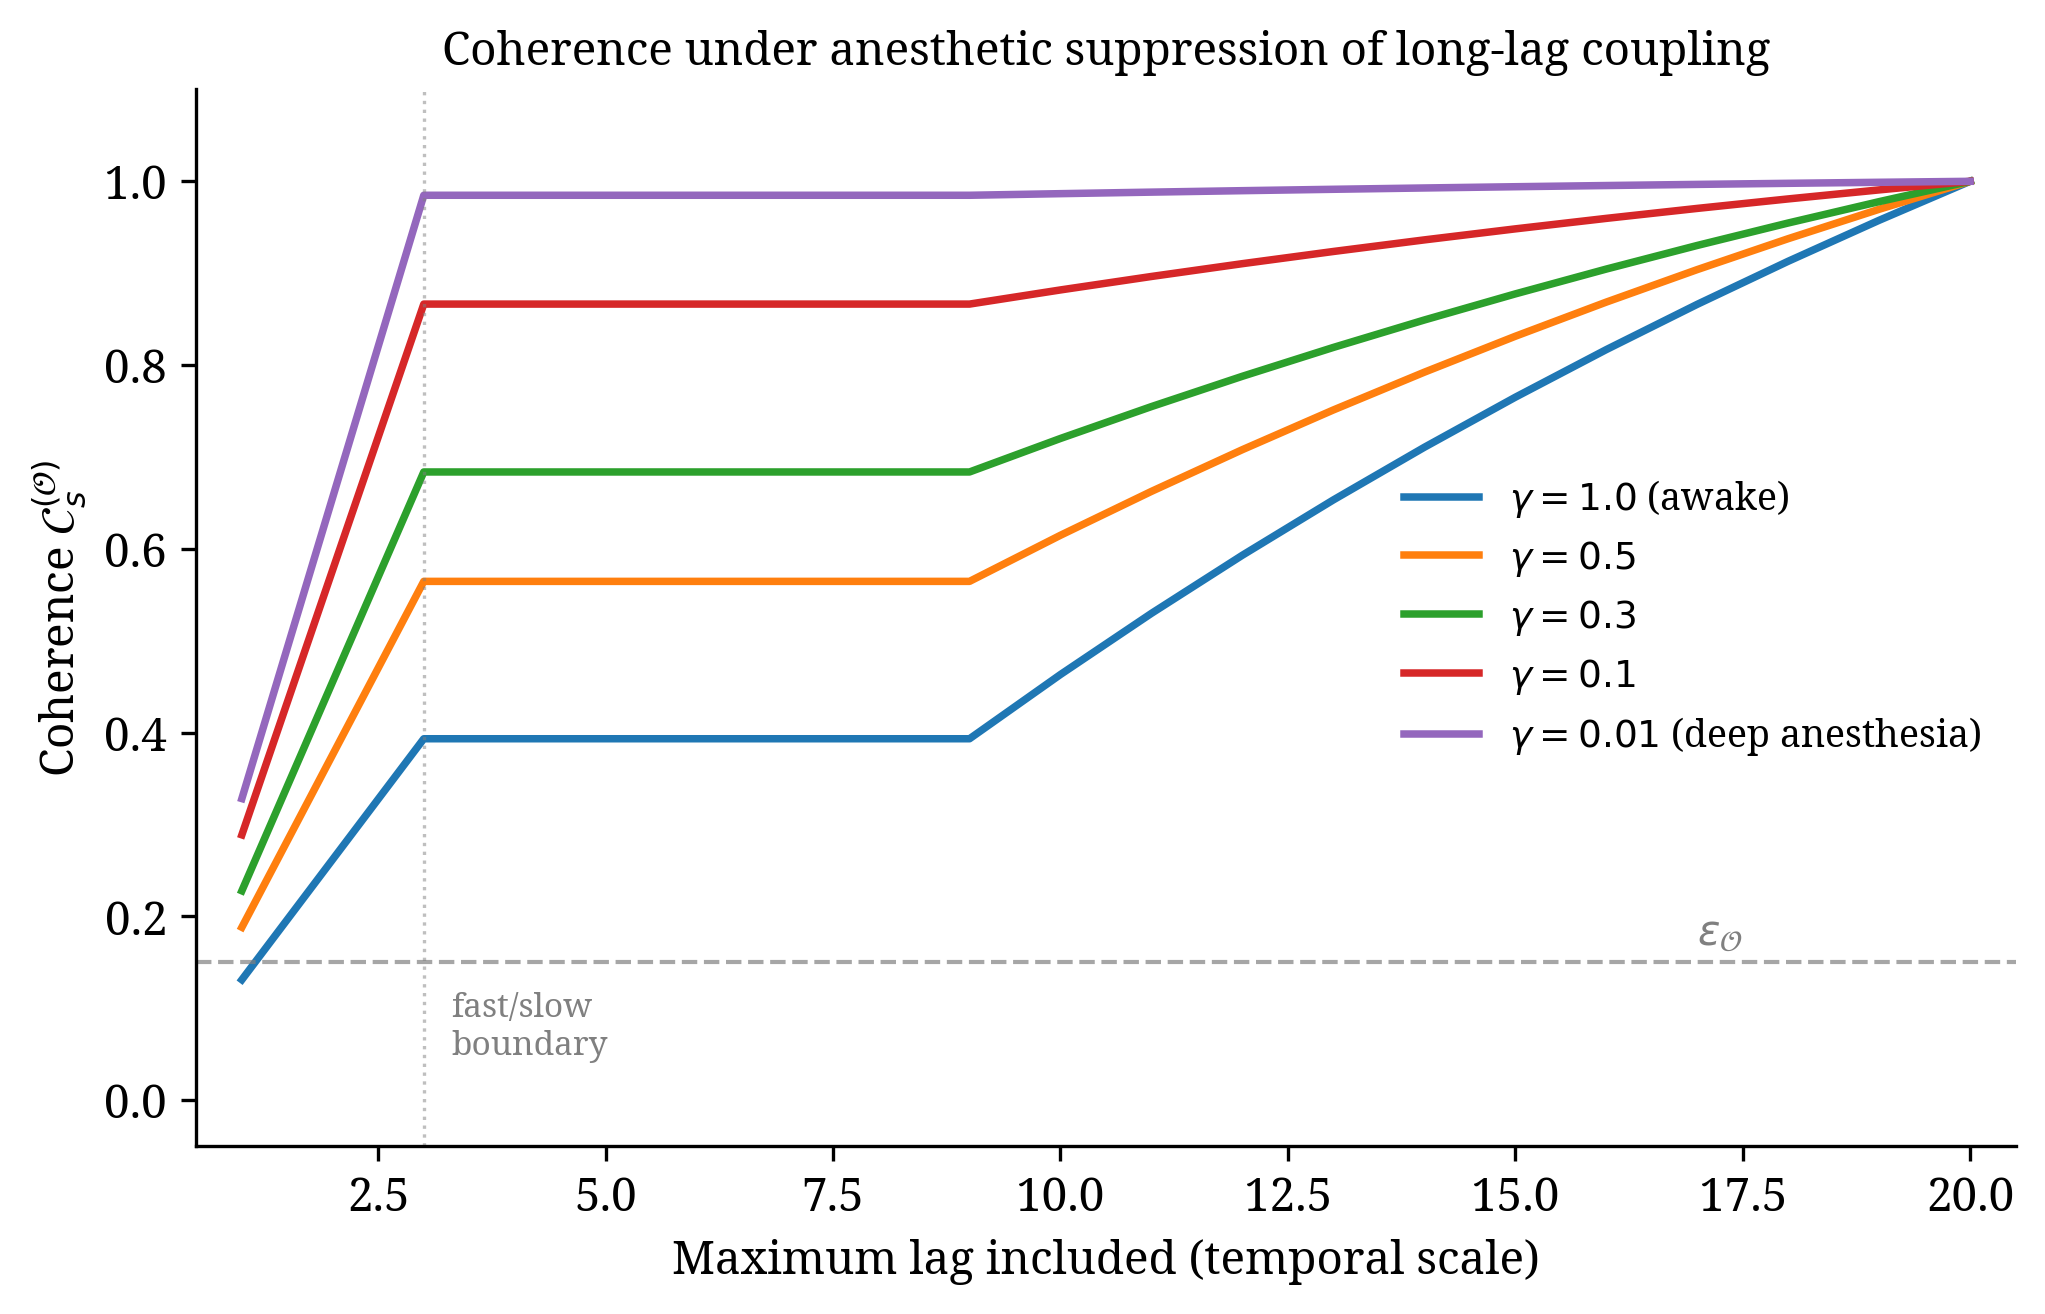
\includegraphics[width=0.8\textwidth]{figures/fig2_neural_suppression.png}
\caption{Neural suppression under anesthesia. The figure illustrates how long lag coupling is suppressed while short lag coupling is preserved, demonstrating that the structure is not annihilated but merely shifted below the macroscopic representability threshold.}
\label{fig:neural}
\end{figure}

\section{Relationship to Existing Frameworks}

To clarify the contribution of this framework, we map it structurally against three prominent existing theories: Integrated Information Theory, the Free Energy Principle, and decoherence based approaches. The key distinction is that these frameworks tend to treat coherence, information, or integration as intrinsic properties of systems, whereas this framework treats them as properties of an observer scale representation triple.

\subsection{Integrated Information Theory (IIT)}
IIT defines a scalar quantity $\Phi$ that measures the integrated information of a system \cite{tononi2016integrated}. It assumes a fixed system boundary and a fixed partition of elements. In our framework, IIT corresponds to a special case where the scale filtration $\mathcal{F}_s$ is held constant, and the interface map $I_{\mathcal{O}}$ is taken to be a faithful embedding of $\mathcal{R}$ into $\Sigma_{\mathcal{O}}$. By relaxing these constraints, our framework allows integration to vary dynamically as the observer scale or interface changes.

The structural difference can be stated precisely. IIT treats $\Phi$ as a property of the system itself. In our framework, the analogous quantity $\mathcal{I}[x]$ is a property of the observer system interaction. Two observers with different interface maps will in general compute different values of $\mathcal{I}[x]$ for the same underlying state $r \in \mathcal{R}$. IIT does not account for this observer dependence because it does not parameterize the observer.

\subsection{The Free Energy Principle (FEP)}
The FEP posits that biological systems maintain their structure by minimizing variational free energy, which requires a Markov blanket to separate the agent from the environment \cite{friston2010free}. The FEP variational free energy can be viewed as a special case of our scale conditioned information $\mathcal{I}_s[x]$ evaluated at a single, fixed scale. Our framework does not require the a priori existence of a Markov blanket; rather, the boundary between observer and environment is dynamically generated by the interface map $I_{\mathcal{O}}$.

\subsection{Decoherence Theory}
In quantum mechanics, decoherence describes the loss of coherence when a system interacts with its environment \cite{zurek2003decoherence}. Let $\mathcal{H}_S \otimes \mathcal{H}_E$ denote the joint Hilbert space of the system and environment. Decoherence is a physical mechanism specific to quantum substrates. Our framework is substrate neutral. What decoherence theory describes as the irreversible tracing out of environmental degrees of freedom, our framework describes as a scale filtration where the fine grained correlations are no longer representable by the macroscopic observer.

\subsection{Summary of Structural Differences}

The following table summarizes the key structural differences between the present framework and the three comparison theories.

\begin{table}[ht]
\centering
\begin{tabular}{|l|c|c|c|c|}
\hline
\textbf{Property} & \textbf{This framework} & \textbf{IIT} & \textbf{FEP} & \textbf{Decoherence} \\
\hline
Observer parameterized & Yes & No & Partial & No \\
\hline
Scale relative coherence & Yes & No & No & Partial \\
\hline
Substrate neutral & Yes & Yes & Yes & No \\
\hline
No fixed boundary & Yes & No & No & No \\
\hline
No inference architecture & Yes & Yes & No & Yes \\
\hline
Domain generality & High & Medium & Medium & Low \\
\hline
\end{tabular}
\caption{Structural comparison of the present framework with IIT, FEP, and decoherence theory.}
\label{tab:comparison}
\end{table}

\begin{figure}[ht]
\centering
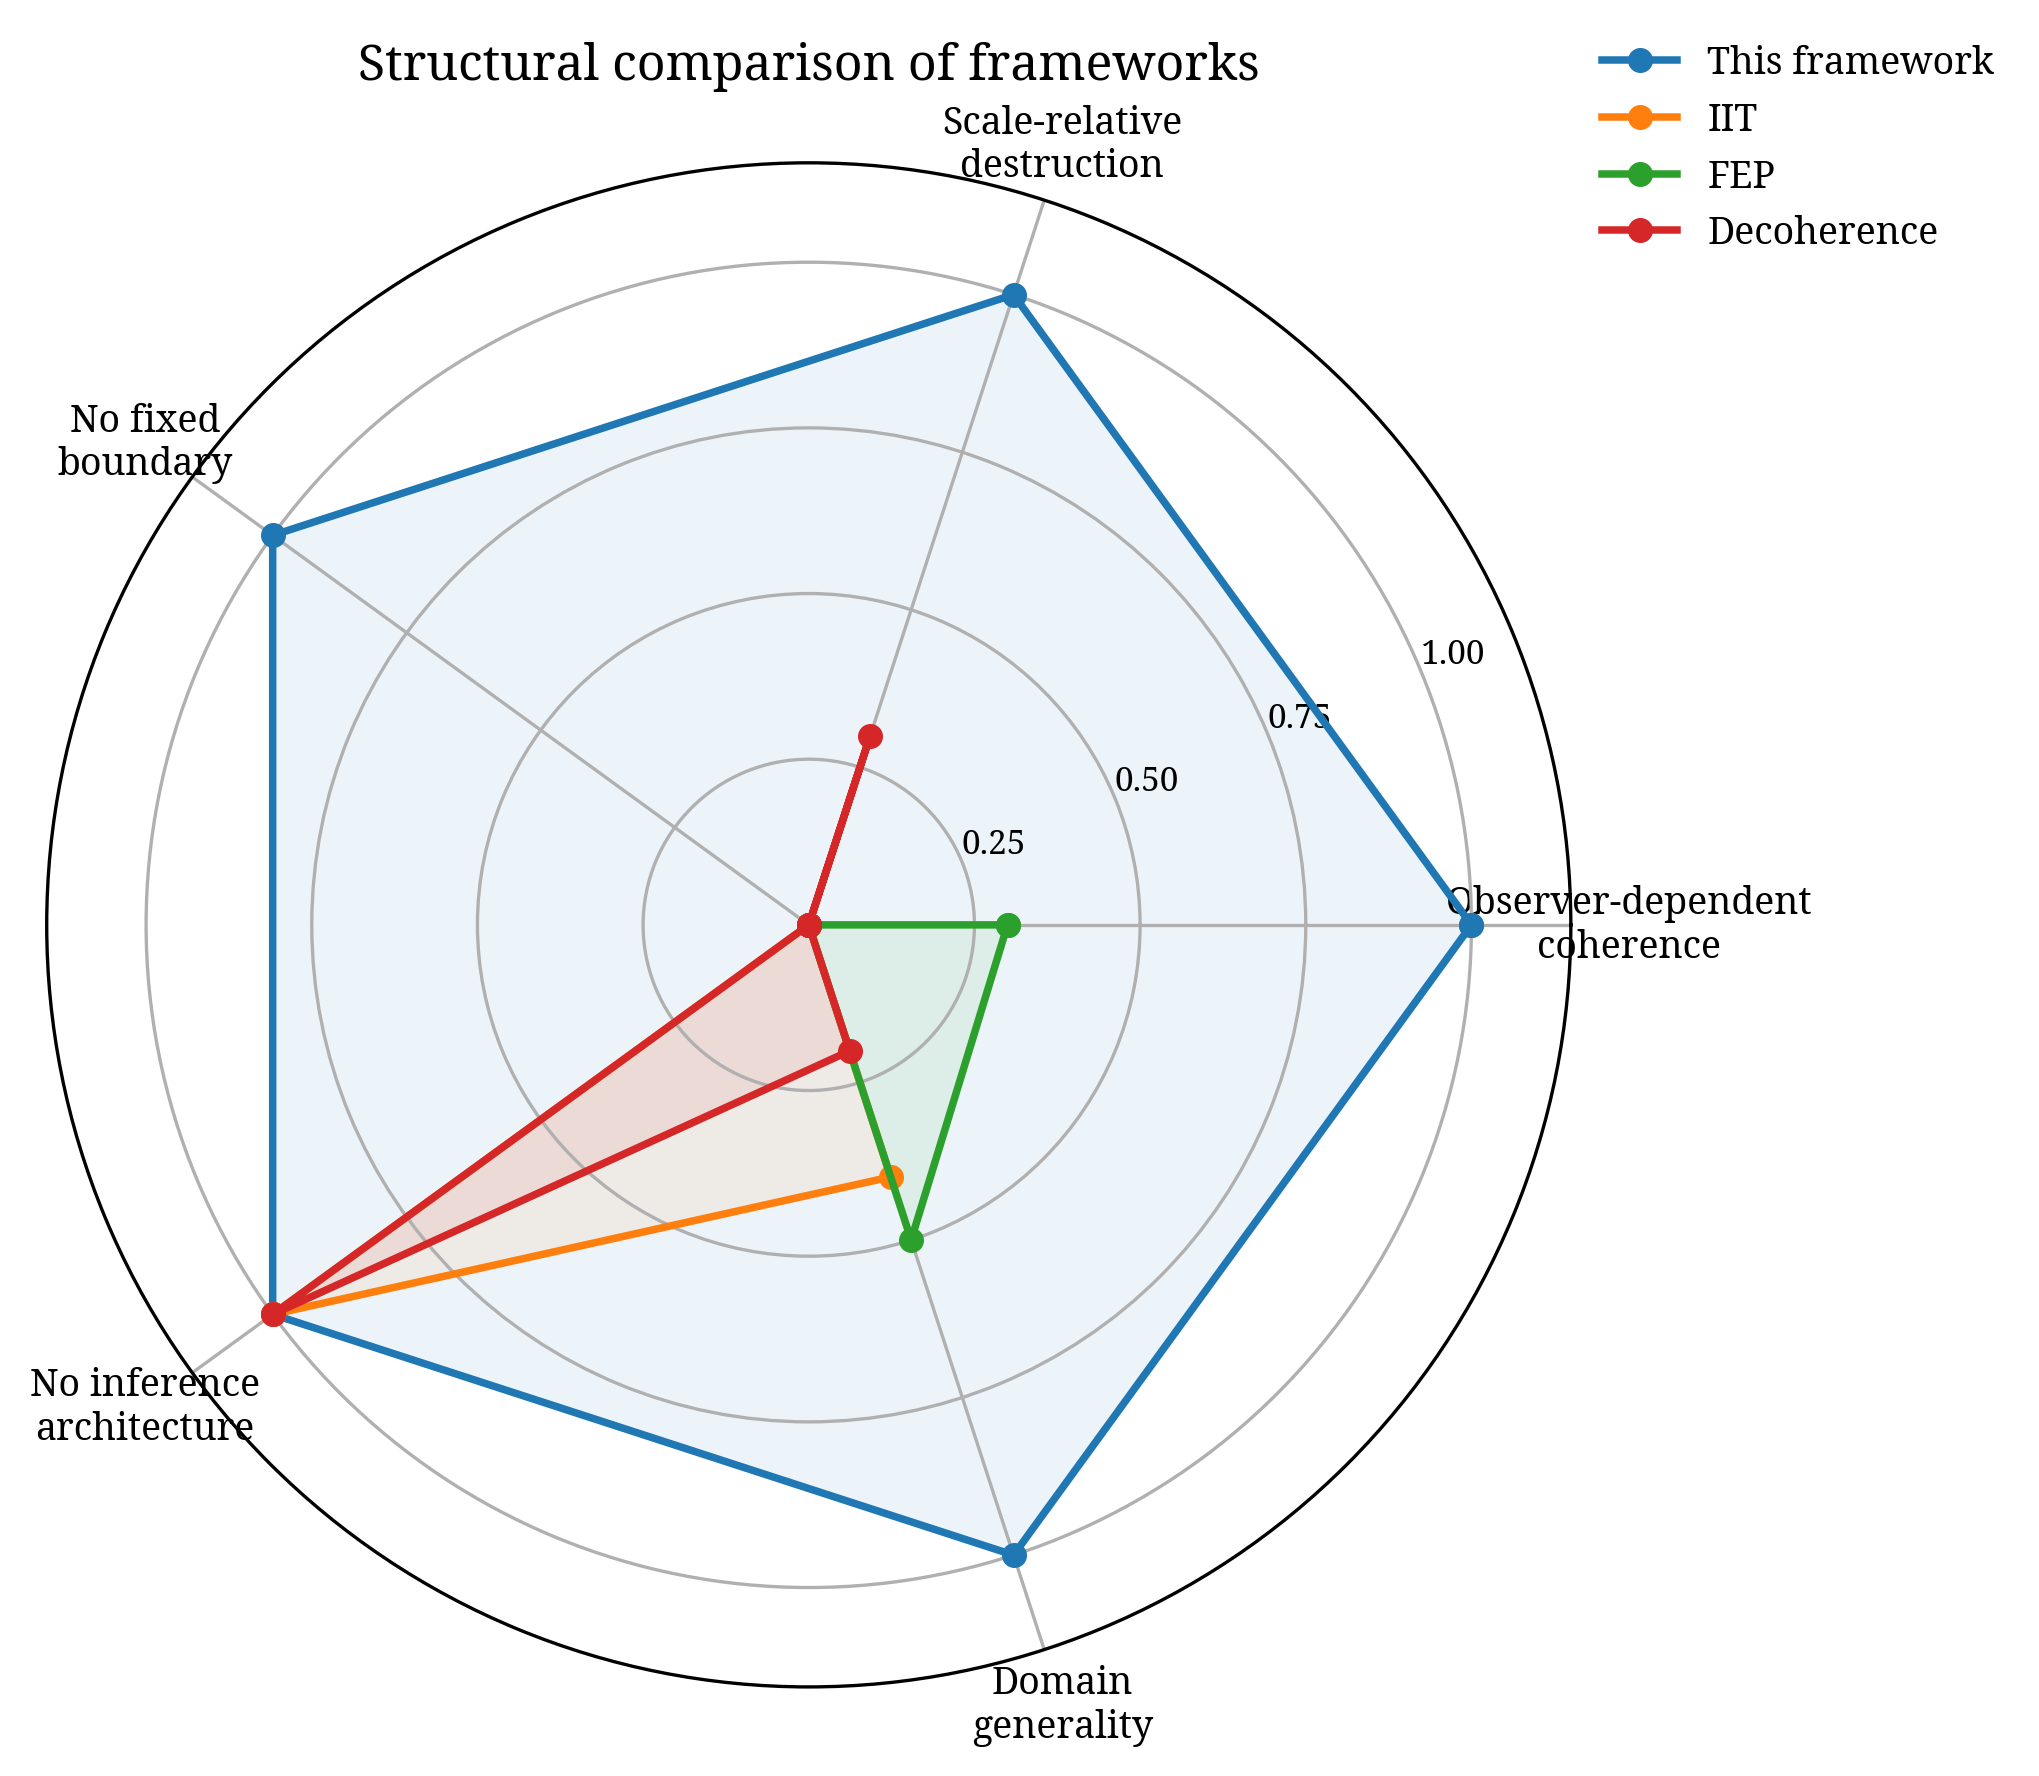
\includegraphics[width=0.8\textwidth]{figures/fig4_framework_comparison.png}
\caption{Framework comparison radar chart. This visualizes the structural differences between the present framework, IIT, FEP, and Decoherence across key dimensions such as observer dependence, scale relativity, and substrate neutrality.}
\label{fig:frameworks}
\end{figure}

\section{Computability and Tractable Approximation}

The integrated relational information $\mathcal{I}[x]$ is generally computationally intractable or statistically difficult to estimate for large systems \cite{paninski2003estimation}. The binding tensor $\mathcal{B}_{ij}(x)$ has $|E|^2$ entries, and estimating each entry from finite data introduces statistical error that compounds across the integration. However, the framework identifies the exact quantity to be approximated and the structural properties that a good approximation must preserve.

\subsection{Sparse Graph Truncation}
For systems where the binding tensor $\mathcal{B}_{ij}$ is sparse (i.e., most pairs of components have negligible relational structure), we can truncate the integration to the non zero or above threshold components. If the binding tensor has at most $m$ non zero entries per row, the computational cost reduces from $O(|E|^2)$ to $O(m \cdot |E|)$. This approximation provides a lower bound on the true information:
\begin{equation}
\mathcal{I}_{\text{sparse}}[x] = \int_{E \times E} \mathcal{B}_{ij}(x) \cdot \mathbf{1}_{\{\mathcal{B}_{ij}(x) > \tau\}} \, d\nu(i,j) \leq \mathcal{I}[x]
\end{equation}
where $\tau$ is a sparsity threshold.

\subsection{Low Rank Approximation}
Let $\mathcal{I}^{(k)}$ denote the approximation induced by truncation to $k$ principal components of the binding tensor. If the binding tensor has a rapidly decaying spectrum, the first $k$ components capture the dominant relational structure. This provides a tractable lower bound on the true information. The notation $\mathcal{I}^{(k)}$ is local to this section and should not be confused with the scale conditioned information $\mathcal{I}_s[x]$.

\subsection{Windowed Transfer Entropy}
For time series data (as in Example 2), windowed transfer entropy provides a localized estimate of the binding tensor \cite{schreiber2000measuring}. The window length determines the temporal resolution of the estimate. For bias corrected estimators, windowed transfer entropy converges to the true value under standard regularity conditions; without correction, estimates may be biased \cite{paninski2003estimation}.

\subsection{Structural Properties of Approximations}
A good approximation must preserve three structural properties: (P1) it must be a lower bound on the true information, ensuring that any coherence detected in the approximation is real; (P2) it must respect the scale filtration, meaning the approximation at coarser scales is less than or equal to the approximation at finer scales; (P3) it must preserve the monotonicity of the coherence functional. Both sparse truncation and low rank approximation satisfy these properties.

These approximations ensure that the framework can be applied to empirical data, such as EEG recordings or simulated physical systems, without requiring infinite computational resources. The framework does not claim to be easy to compute; it claims to identify the correct quantity and the structural constraints that any tractable approximation must satisfy.

\section{Discussion}

The framework presented here shifts the locus of mathematical and informational structure from the absolute reality to the observer interface. By doing so, it resolves the paradox of apparent destruction. When a system undergoes a radical transformation, its structure is not annihilated; it is redistributed into a form that is no longer coherent at the observer original scale.

This reframing has several concrete consequences. First, it provides a principled way to distinguish between what is lost and what is merely hidden. In the statistical mechanics example, marginalizing out degrees of freedom reduces the observable coherence, but the underlying correlations persist in the full state space. In the neuroscience example, anesthesia suppresses macroscopic cortical coupling, but the local, high frequency structure remains intact. In both cases, the framework correctly identifies the transformation as apparent destruction rather than absolute annihilation.

Second, the framework provides a formal language for comparing different theoretical approaches. By mapping IIT, the Free Energy Principle, and decoherence theory into the observer interface framework, we can identify exactly where each theory makes implicit assumptions about the observer, the scale, or the system boundary. IIT assumes a fixed partition and no observer. The FEP assumes a Markov blanket and a single scale. Decoherence theory assumes a quantum substrate. Our framework makes none of these assumptions, which is both its strength and its limitation: it is more general, but it requires more structure to be specified before it can be applied to a concrete system.

Third, the proof of emergent universality (Theorem 5) demonstrates that we do not need to posit a Platonic realm of mathematical objects to explain why different observers agree on mathematical truths. The agreement is a necessary consequence of overlapping interfaces interacting with a shared reality. This is not a philosophical argument; it is a mathematical theorem with explicit hypotheses (finite family, pairwise non singularity, compatible filtrations) and a constructive proof.

Finally, the dynamics of observer evolution (Section 6) open a new direction for formal epistemology. Learning, in this framework, is not the accumulation of facts but the refinement of the observer interface. When an observer refines its scale filtration, it gains access to structure that was previously below its representability threshold. This provides a formal model of scientific progress: the history of science can be understood as the progressive refinement of observer interfaces, each refinement expanding the formal system and bringing previously hidden structure into representability.

\section{Limitations and Future Work}

The current framework has several limitations that should be stated explicitly.

First, the proof of emergent universality (Theorem 5) is restricted to finite families of observers. Extending this to infinite families requires additional topological or measure theoretic compactness conditions on the space of observer interfaces. Without such conditions, the intersection of infinitely many formal systems could be empty even if every finite sub intersection is non empty. This is a genuine mathematical gap, not merely a technical inconvenience.

Second, the dynamics of observer evolution (Section 6) were analyzed primarily under pure scale refinement, with the binding tensor, index space, and measure held fixed. A full theory of observer dynamics must account for simultaneous changes in the sensor set, partition map, compression map, and transformation set. In particular, sensor evolution (where the observer gains access to entirely new channels of information) is qualitatively different from scale refinement and may not preserve the monotonicity properties established in Theorem 7.

Third, the examples presented here are idealized. The Gaussian statistical mechanics example assumes exact knowledge of the covariance matrix, and the neural systems example assumes stationarity and ergodicity. Real empirical applications will require robust estimation procedures for the binding tensor under non stationary, finite sample conditions.

Fourth, the framework does not currently address the question of observer creation or destruction. We define observer evolution as a map between observer tuples, but we do not formalize the conditions under which a new observer comes into existence or an existing observer ceases to function.

Future empirical work will focus on applying the tractable approximations (Section 10) to high density neural recordings (such as the publicly available datasets from the Human Connectome Project or the Allen Brain Observatory) to track the scale relative persistence of cognitive structures during states of unconsciousness. Future theoretical work will focus on extending the universality theorem to infinite families and developing a full dynamics of observer creation and destruction.

\section{Conclusion}

We have constructed a formal architecture in which coherence, representability, and mathematical systems are emergent properties of an observer interface interaction. The dependency chain from the underlying reality $\mathcal{R}$ through the observer interface $I_{\mathcal{O}}$, binding tensor $\mathcal{B}_{ij}$, scale conditioned information $\mathcal{I}_s[x]$, coherence functional $\mathcal{C}_s^{(\mathcal{O})}[x]$, distinction set $\mathcal{D}_{\mathcal{O}}$, and formal system $\mathfrak{M}_{\mathcal{O}}$ provides a complete, self contained architecture for analyzing the relationship between observer, scale, and structure.

By explicitly parameterizing the observer and the scale of observation, we have shown that apparent destruction is a loss of representability, not absolute annihilation. Theorem 1 establishes that structure persists at some scale under non annihilating transformations. Theorem 2 (the strengthened version) provides a quantitative lower bound on the coherence at the persisting scale. Theorem 3 formalizes the observer relativity of destruction. Theorem 4 establishes the interface dependent ontology.

The cross observer results (Theorems 5 and 6) resolve the problem of mathematical universality without invoking Platonism. The shared formal system $\mathfrak{M}^*$ is not a pre existing mathematical realm; it is the constructive intersection of observer generated formal systems over a shared reality. The dynamics results (Theorems 7 and 8) show that observer evolution through scale refinement is monotonic and convergent.

This framework provides a rigorous, substrate neutral language for analyzing the persistence of complex systems across radical state changes. It grounds the universality of mathematics in the shared structure of observer interfaces rather than in unobservable Platonic ideals. And it opens a new formal direction for understanding how observers, through the refinement of their interfaces, progressively expand the domain of representable structure.

\appendix

\section{Proof Details and Technical Notes}

\subsection{On the Measurability of the Coherence Functional}
The coherence functional $\mathcal{C}_s^{(\mathcal{O})}[x] = \mathcal{I}_s[x] / \mathcal{I}[x]$ is well defined whenever $\mathcal{I}[x] > 0$. The measurability of $\mathcal{C}_s^{(\mathcal{O})}$ as a function of $x$ follows from the measurability of the binding tensor $\mathcal{B}_{ij}(x)$ (assumed in Definition 8), the measurability of conditional expectation (a standard result in measure theory), and the measurability of the ratio of two measurable functions on the set where the denominator is non zero.

\subsection{On the Least Fixed Point Construction}
The formal system $\mathfrak{M}_{\mathcal{O}}$ is defined as the least fixed point of a set operation (Definition 15). The existence of this least fixed point is guaranteed by the Knaster Tarski theorem, which states that every monotone function on a complete lattice has a least fixed point. The relevant lattice here is the power set of $\Sigma_{\mathcal{O}}$, ordered by inclusion. The set operation $X \mapsto \mathcal{V}_{\mathcal{O}} \cup \{T(x) : x \in X, T \in \mathcal{T}_{\mathcal{O}}\}$ is monotone because adding elements to $X$ can only increase the set of states reachable by admissible transformations.

\subsection{On the Tower Property in Lemma 1}
The proof of Lemma 1 relies on the tower property of conditional expectation: if $\mathcal{G}_1 \subseteq \mathcal{G}_2$ are sub $\sigma$-algebras, then $\mathbb{E}[\mathbb{E}[X | \mathcal{G}_2] | \mathcal{G}_1] = \mathbb{E}[X | \mathcal{G}_1]$. This is a standard result that holds for any integrable random variable $X$. In our context, $X = \mathcal{B}_{ij}(x)$, $\mathcal{G}_1 = \mathcal{F}_{s_2}$ (coarser), and $\mathcal{G}_2 = \mathcal{F}_{s_1}$ (finer). The decomposition follows by writing $\mathbb{E}[\mathcal{B}_{ij} | \mathcal{F}_{s_1}] = \mathbb{E}[\mathcal{B}_{ij} | \mathcal{F}_{s_2}] + (\mathbb{E}[\mathcal{B}_{ij} | \mathcal{F}_{s_1}] - \mathbb{E}[\mathcal{B}_{ij} | \mathcal{F}_{s_2}])$ and integrating over $E \times E$.

\subsection{On the Monotonicity of Coherence}
The proof of Theorem 3 uses the claim that $\mathcal{C}_s^{(\mathcal{O})}[x]$ is non increasing in $s$. This follows from the fact that $\mathcal{I}_s[x]$ is non increasing in $s$ (because conditioning on a coarser $\sigma$-algebra cannot increase the conditional expectation of a non negative quantity) while $\mathcal{I}[x]$ is independent of $s$. The ratio is therefore non increasing.

\subsection{Simulation Notes}
The figures in this paper were generated using Python with Matplotlib. All code is available in the accompanying repository. Figure 1 computes the Gaussian mutual information for a system of 3 and 2 variables with uniform pairwise correlation $\rho$, demonstrating the coherence drop under marginalization. Figure 2 models the neural suppression scenario with 20 cortical sites and a lag dependent suppression factor. The radar chart in Figure 4 compares the present framework against IIT, FEP, and decoherence across five structural dimensions. Figure 3 shows the definition dependency chain.

\section{Notation Index}

For reference, we provide a complete index of the notation used in this paper, organized by the section in which each symbol is first introduced.

\begin{table}[ht]
\centering
\begin{tabular}{|l|l|l|}
\hline
\textbf{Symbol} & \textbf{Meaning} & \textbf{Definition} \\
\hline
$\mathcal{R}$ & Underlying reality & Def. 1 \\
$\mathcal{O}$ & Observer tuple $(\mathcal{S}, \mathcal{P}, \mathcal{C}, \mathcal{A})$ & Def. 2 \\
$\mathcal{T}_{\mathcal{O}}$ & Admissible transformation set & Def. 3 \\
$I_{\mathcal{O}}$ & Interface map & Def. 4 \\
$\mathcal{R}_{\mathcal{O}}$ & Observer accessible quotient & Def. 5 \\
$\{\mathcal{F}_s\}$ & Scale filtration & Def. 6 \\
$(E, \nu)$ & Component index space & Def. 7 \\
$\mathcal{B}_{ij}(x)$ & Binding tensor & Def. 8 \\
$\mathcal{I}[x]$ & Integrated relational information & Def. 9 \\
$\mathcal{I}_s[x]$ & Scale conditioned information & Def. 10 \\
$\mathcal{C}_s^{(\mathcal{O})}[x]$ & Coherence functional & Def. 11 \\
$\epsilon_{\mathcal{O}}$ & Coherence threshold & Def. 12 \\
$\mathcal{D}_{\mathcal{O}}$ & Distinction set & Def. 13 \\
$\mathcal{V}_{\mathcal{O}}$ & Invariant set & Def. 14 \\
$\mathfrak{M}_{\mathcal{O}}$ & Observer relative formal system & Def. 15 \\
$\Psi_{\mathcal{O}}$ & Representability map & Def. 16 \\
$\alpha$ & Information non annihilation parameter & Def. 17 \\
$\beta$ & Bounded scale distortion parameter & Def. 18 \\
$\mathcal{J}(\mathcal{O}_1, \mathcal{O}_2)$ & Joint representability set & Def. 19 \\
$\mathfrak{M}_{\mathcal{O}_1 \cap \mathcal{O}_2}$ & Shared formal system & Def. 20 \\
$\Omega(\mathcal{O}_1, \mathcal{O}_2)$ & Observer overlap & Def. 24 \\
$\Xi$ & Observer evolution map & Def. 25 \\
$\Delta\Psi$ & Representability expansion & Def. 26 \\
$\nabla\Psi$ & Representability contraction & Def. 27 \\
$\gamma$ & Neural suppression parameter & Example 2 \\
\hline
\end{tabular}
\caption{Complete notation index with definition numbers.}
\label{tab:notation}
\end{table}

\bibliographystyle{plain}
\bibliography{references}

\end{document}
